%\documentclass{article}

%,twocolumn

\documentclass[aps,prd,showpacs,superscriptaddress,groupedaddress]{revtex4-1}  % for review and submission
%\documentclass[aps,preprint,showpacs,superscriptaddress,groupedaddress]{revtex4}  % for double-spaced preprint
\usepackage{graphicx}  % needed for figures
\usepackage{dcolumn}   % needed for some tables
\usepackage{bm}        % for math

%%%%%%%%%%%%%%%%%%%%%%%%%%%%%%%%%%%%%%%%%%%%%%%%%%%%%%%%%%%%%%%%%%%%%%%%%%%%%%%%%%%%%%%%%%%%%%%%%%%%%%%%%%%%%%%%%%%%%%%%%%%%
\usepackage{amsfonts}
\input{journals_list.txt}

\usepackage{amssymb,latexsym,amssymb,amsmath,amsbsy,amsopn,amstext,upgreek}
\usepackage{color}
\usepackage{graphicx,wrapfig,fancybox,watermark,graphics}
\usepackage{pgf}
\usepackage{float}

\usepackage{vmargin}
\usepackage{cjhebrew}
\usepackage{subfigure}
\usepackage[toc,page]{appendix}


% avoids incorrect hyphenation, added Nov/08 by SSR
\hyphenation{ALPGEN}
\hyphenation{EVTGEN}
\hyphenation{PYTHIA}


\newcommand{\homeLinux}{/home/yabebal/}
\newcommand{\homeMac}{/Users/yabebal/}
\newcommand{\home}{\homeLinux}

\newcommand{\figdir}[1]{figures/#1}


\def\rms{root mean square~}
\newcommand{\figref}[1]{Figure (\ref{#1})}
%\newcommand{\eqref}[1]{Eqn. (\ref{#1})}
\newcommand{\reffig}[1]{Figure (\ref{#1})}
\newcommand{\refeq}[1]{Eqn. (\ref{#1})}
\newcommand{\refsec}[1]{Section \ref{#1}}
\newcommand{\secref}[1]{Section \ref{#1}}
\newcommand{\healpix}{HEALpix~}
\newcommand{\nside}[1]{N_{\rm side}}


\begin{document}

\title{A Numerical Investigation on the High-Frequency Geometry of Spherical Random Eigenfunctions\thanks{%
Research supported by ERC Grant 277742 Pascal.}}
\author{Yabebal Fantaye}
\affiliation{African Institute for Mathematical Sciences and Stellenbosch University, Cape Town, South Africa}
\author{Valentina Cammarota}
\affiliation{Department of Statistics, Sapienza University of Rome}
\author{Domenico Marinucci}
\affiliation{Dipartimento di Matematica, Universit\'{a} di Roma
''Tor Vergata'', Via della Ricerca Scientifica 1, I-00133 Roma,
Italy}
\author{Anna Paola Todino}
\affiliation{Gran Sasso Science Institute, L'Aquila, Italy}


%{Authors}

\date{\today}



\begin{abstract}
A lot of attention has been drawn over the last few years by the investigation of the geometry of spherical random eigenfunctions (random spherical harmonics) in the high frequency regime, i.e ., for diverging eigenvalues. In this paper, we present a review of these results and we collect for the first time a comprehensive numerical investigation, focussing on particular on the behaviour of Lipschitz-Killing curvatures/Minkowski functionals (i.e., the area, the boundary length and the Euler-Poincar\'e characteristic of excursion sets) and on critical points. We show in particular as very accurate analytic predictions can be given for their expected values and variances, for the correlation among these functionals, and for the cancellation that occurs for some specific thresholds (the variances becoming an order of magnitude smaller - the so-called Berry's cancellation phenomenon). Most of these functionals have very important statistical applications, for instance in connection to the analysis of Cosmic Microwave Background data.
\end{abstract}

\keywords{CMB, Data Analysis, Minkowski Functionals,
Gaussian Kinematic Formula, Spherical Harmonics}

\pacs{98.80.Es, 95.75.Mn, 95.75.Pq, 02.50.-r}

% 98.80.Es     Observational cosmology
% 95.75.Mn     Image processing
% 95.75.Pq     Mathematical procedures and computer techniques
% 02.50.-r Statistics

\maketitle

\section{Introduction}

The geometry of the excursion sets for random fields on the sphere has been the object of rather intense research over the last decade or so. For any real number $u$, the excursion sets of a random field $f(x)$ are defined by%
\begin{equation}
A_{u}(f):=\left\{ x:f(x) \geq u\right\} \text{ ,}
\end{equation}
or, more explicitly, they represent the subregions where the value of $f$ exceeds the threshold $u$. It is well-known that these geometrical properties can be characterized in terms of the so-called Lipschitz-Killing curvatures (or equivalently, Minkowski functionals), which in the two dimensional case correspond to the excursion area, (half) the boundary length and the Euler-Poincar\'e characteristic (connected regions minus number of holes) of the excursion set. A comprehensive description of Lipschitz-Killing curvatures for excursion sets of random fields is given in the excellent monograph by Adler and Taylor .....; ; these functionals can be computed on real data by means of
accurate and numerically efficient algorithms \cite{KLENK2006127, Guderlei2007, Gay2012_NGPeaks}. These functionals have been widely applied in the analysis of experimental data, especially in a Cosmological framewrok, see i.e.,  \cite{natoli2010mfBoomrang, matsubara2010_mfFnl,
  ducout2013_mfFnl, gratten2012_mfLSSreview, munshi2013_mfSkewCl,planck2013_IS, planck2014-a18} and the references therein.


A lot of mathematical efforts have been spent since the '80s on the characterization of expected values of these functionals under Gaussianity, culminating in the discovery of the beautiful Gaussian Kinematic Formula \cite{TaylorAdler2009}; comparing these expected values with realization allows the implementation of a number of tests for Gaussianity and Isotropy (see again \cite{planck2013-p09, planck2014-a18}).

While the behaviour of expected values is now fully understood, it is clear that the implementation of more sophisticated, hence more sensitive, testing procedures requires further knowledge, in particular the variance of these functionals and therefore the possibility to establish Central Limit Theorems with correct normalization factors. Establishing a Central Limit result requires of course the exploitation of a suitable notion of asymptotic behaviour; in the framework of spherical fields, the only relevant notion seems to be the one of High-Frequency asymptotics. In particular it is well-known that isotropic random fields on the sphere can be decomposed by means of the Spectral representation theorem into the sum of orthogonal components, each of them corresponding to a different multipole $\ell$. The variance of Minkowski functionals/Lipschitz-Kiling curvatures in the high-frequency/high energy limit has been studied by several authors in recent years, starting from Wigman2009 for the nodal length, and then including, among others, Nazarov and Sodin...for the number of connected components, MWigman2011 for the excursion area, MWigman 2014 for the Defect, CammarotaMWigman for the Euler-Poincarè characteristic, MRossiWigman for the distribution of the nodal length, CammarotaMWigman... for the critical values and CammarotaWigman for the total number of critical points, CammarotaMarinucci2016,2018, see also Dalmao, Nourdin,Peccati, MPRW, Maffucci,.....for related works covering also the 2-dimensional torus....\cite{cm1603}.


Our aim in this paper is to present a unified overview of this literature, and especially to perform a detailed numerical investigation to verify the practical relevance of these results when investigating spherical Gaussian maps. We shall address several issues concerning not only the expected value and variances of these functionals, but also their cross-correlation across different level sets. The theoretical predictions which have so far been produced are validated for the first time from a numerical point of view, and moreover their domain of applicability is clarified. Indeed, in terms of the variances the theoretical expressions which are obtained should be viewed as leading terms in series expansions of the variances over different "chaos" components; as such, the approximation depends on the speed of convergence to zeroes of the terms which are dropped. This speed is known to be polynomial in some cases (namely, those corresponding to non-zero levels) and logarithmic in others (those corresponding to zero levels); this duality is mirrored in the numerics we present.



Minkowski Functionals are not the only objects of interest in this paper. Indeed, some other recent contributions have derived neat analytic formulae for the expected number and the variance of critical points on the same spherical harmonics components as considered earlier for MFs \cite{cm1603}. In this paper, we are exploiting these results for the first time as a further tool to search for residual point sources.   


The plan of the paper is as follows: in Section 2, we review the results on the expected values and variances for the Lipschitz-Kiling Curvatures; in Section 3 we discuss the behaviour of critical points, again revieweing the analytic results that are currently available, while Section 4 is devoted to the analysis of the correlation among these different functionals. Section 5 describes our implementation algorithms and presents the numerical results; we then draw some some conclusions and present directions for future work.

\section{Characterization of Excursion Sets for Random Spherical Harmonics}

In the case of the two-dimensional sphere, the excursion sets $A_{u}(f)$ of a given (possibly random)
function $f$ are defined as
\begin{equation}
A_{u}(f):=\left\{ x\in \mathbb{S}^{2}:f(x)\geq u\right\} \text{ .}
\end{equation}
Of course, in the limit where we take $u=-\infty ,$ we have that $%
A_{u}(f)=S^{2}$. In this paper, we shall be concerned with random eigenfunctions which satisfy the Helmhotz equation @@@per favore anna paola, inserisci l'equazione, e specifica che prendiamo autofunzioni normalizzate per avere varianza 1!!!! grazie

\begin{equation*}
\Delta _{\mathbb{S}^{2}}f_{\ell }+\lambda _{\ell }f_{\ell }=0,\mbox{ }\mbox{
}\mbox{ }f_{\ell }:\mathbb{S}^{2}\rightarrow \mathbb{R},
\end{equation*}%
where $\Delta _{\mathbb{S}^{2}}$ is the Laplace-Beltrami operator on $%
\mathbb{S}^{2}$, defined as usual as
\begin{equation*}
\dfrac{1}{\sin \theta }\dfrac{\partial }{\partial \theta }\bigg\{\sin \theta 
\dfrac{\partial }{\partial \theta }\bigg\}+\dfrac{1}{\sin ^{2}\theta }\dfrac{%
\partial ^{2}}{\partial \varphi ^{2}},\mbox{ }0\leq \theta \leq \pi ,\mbox{ }%
0\leq \varphi < 2\pi ,
\end{equation*}%
and $\lambda _{\ell }=\ell (\ell +1),\mbox{ }\ell =0,1,\dots $. For a given
eigenvalue $\lambda _{\ell },$ the corresponding eigenspace is the $(2\ell
+1)-$dimensional space of spherical harmonics of degree $\ell .$
The random fields $\{f_{\ell }(x),x\in \mathbb{S}^{2}\}
$ are Gaussian and isotropic. %From the addition theorem for spherical harmonics, 
Also, we have that 
\begin{eqnarray*}
	\mathbb{E}[f_{\ell }(x)] &=&0,\mbox{ and }\mathbb{E}[f_{\ell }(x)^{2}]=1%
	\text{,} \\
	\mathbb{E}[f_{\ell }(x)f_{\ell }(y)] &=&P_{\ell }(\cos d(x,y)),
\end{eqnarray*}%
where $P_{\ell }$ are the Legendre polynomials and $d(x,y)$ is the spherical
geodesic distance between $x$ and $y,$ i.e. 
\begin{equation*}
d(x,y)=\arccos (\langle x,y\rangle ).
\end{equation*}%




@@@@

In this paper we aim at the implementation of Minkowski functionals/Lipschitz-Killing curvatures (to be defined below) on the spherical harmonic/Fourier components of of observed data. Let us first recall the well-known spectral representation theorem for spherical random fields, which states that the following identity holds, in the $L^2$ sense:
\begin{equation}
f(x)=\sum_{\ell =1}^{L_{\max }}\sum_{m=-\ell }^{\ell }a_{\ell m}Y_{\ell
m}(x)=\sum_{\ell =1}^{L_{\max }}f_{\ell }(x)\text{ ;}  \label{specrap}
\end{equation}%
The spherical harmonic coefficients may be computed from the field $f(.)$ by means of the inverse transform

\begin{equation}
a_{\ell m}= \int_{S^2} f(x) \bar{Y}_{\ell
m}(x)dx, \text{ } \text{ } \ell =1,2,...., m=-\ell,...,\ell ,   \label{specrap2}
\end{equation}%

The inverse transform \eqref{specrap2} is only feasible for unmasked (full-sky) data, a condition which is usually considered rather difficult to meet for astrophysical experiments such as those concerning CMB. Rather recently, however, full-sky maps were produced for instance by \cite{starketal2014} and by the Planck collaboration in its 2018 release (see .....). 

%\begin{equation*}
%A_{I}(f_{\ell }; {\cal S}^2):=\left\{ x\in S^{2}:f_{\ell }(x)\in I \right\}.
%\end{equation*}
%For $I=[u,\infty)$, we have 
%\begin{equation*}
%A_{u}(f_{\ell }; {\cal S}^2):=\left\{ x\in S^{2}:f_{\ell }(x) \ge u \right\}.
%\end{equation*}


Let us now recall again the definitions of the \emph{Lipschitz-Killing Curvatures} (LKCs), which correspond to Minkowski functionals up to a different indexing and normalization factors; in two dimensions, they are given by  (a) the Euler-Poincar\'{e} characteristic (written $\mathcal{L}_{0}(A_{u}(f))$), e.g. the number of connected
regions minus the number of holes, or two minus the genus; (b) half the boundary length of
the excursion regions (written $\mathcal{L}_{1}(A_{u}(f))$); the area of the excursion
regions (written $\mathcal{L}_{2}(A_{u}(f))$), which corresponds to the first Minkowski functional. The expected values of these functionals when evaluated on the excursion sets of Gaussian fields has been fully characterized by the Gaussian Kinematic Formula (GKF), see \cite{TaylorAdler2009}. 

We now need the family of functions $\rho _{l}(u)$ defined as
\begin{equation}
\rho _{l}(u)=(2\pi )^{-(l+1)/2}H_{l-1}(u)e^{-u^{2}/2}\text{ ,}
\end{equation} where $H_{k}(u)$ denotes as usual the family of Hermite polynomials, that is,
\begin{equation}
H_{0}(u)=1, H_{1}(u)=u, H_{2}(u)=u^{2}-1;
\end{equation}
it is convenient to define also
\begin{equation}
H_{-1}(u)=\sqrt{2\pi }(1-\Phi (u))e^{u^{2}/2},
\end{equation}
where $\Phi (u)$ is the Gaussian cumulative distribution function, whence%
\begin{eqnarray}
\rho _{0}(u) &=&(2\pi )^{-1/2}\sqrt{2\pi }(1-\Phi
(u))e^{u^{2}/2}e^{-u^{2}/2}=(1-\Phi (u)) \\
\rho _{1}(u) &=&\frac{1}{2\pi }e^{-u^{2}/2}\text{ , }\rho _{2}(u)=\frac{1}{%
\sqrt{(2\pi )^{3}}}ue^{-u^{2}/2}.
\end{eqnarray}%
Adler and Taylor \cite{TaylorAdler2009} write these components $\mathcal{M}_{k}([u,\infty ))=\frac{1}{\sqrt{2\pi }}%
H_{k}(u)e^{-u^{2}/2}$ and denote them Gaussian Minkowski functionals. The so-called "flag" coefficients are instead given by
\begin{equation}
\left[
\begin{array}{c}
i+l \\
l%
\end{array}%
\right] =\left(
\begin{array}{c}
i+l \\
l%
\end{array}%
\right) \frac{\omega _{i+l}}{\omega _{i}\omega _{l}}\text{ , for }\omega
_{i}=\frac{\pi ^{i/2}}{\Gamma (\frac{i}{2}+1)}\text{ ,}
\end{equation}%
that is, $\omega _{i}$ represents the area of the $i-$dimensional unit ball, $%
\omega _{1}=2,$ $\omega _{2}=\pi ,$ $\omega _{3}=\frac{4}{3}\pi.$
As a last ingredient, we write $\lambda$ for the parameter which represents the second derivative of
the covariance function at the origin.

We are now ready to present the general expression for the expected value of Lipschitz-Killing curvature, i.e., the Gaussian Kinematic Formula which reads (Theorem 13.2.1 in \cite{RFG}:

\begin{equation}
\lambda ^{i/2}\mathbb{E}\mathcal{L}_{i}(A_{u}(f(x),D))=\sum_{l=0}^{\dim
(D)-i}\left[
\begin{array}{c}
i+l \\
l%
\end{array}%
\right] \lambda ^{(i+l)/2}\rho _{l}(u)\mathcal{L}_{i+l}(D)\text{ .}
\label{GKF}
\end{equation}


%\subsection{Multipole fields}
As an application of the previous result, let us consider the Fourier components $\{f_\ell(\cdot)\}_{\ell=1,2,\dots}$ normalized to have variance one, the GKF yields immediately (compare
\cite{MarVad}, Corollary 5)%

\begin{equation}
\mathbb{E}\mathcal{L}_{0}(A_{u}(f_{\ell }(.),\mathbb{S}^{2}))=2\left\{ 1-\Phi
(u)\right\} +\frac{\lambda_{\ell}}{2}\frac{ue^{-u^{2}/2}}{\sqrt{(2\pi )^{3}}}%
4\pi \text{ ;}  \label{sh1}
\end{equation}
\begin{equation}
\mathbb{E}\mathcal{L}_{1}(A_{u}(f_{\ell }(.),\mathbb{S}^{2})) =\frac{\pi }{2}%
\frac{1}{\sqrt{2}}\lambda_{\ell}^{1/2}\frac{e^{-u^{2}/2}}{2\pi }%
4\pi=\frac{\pi}{\sqrt{2}} \lambda_{\ell}^{1/2}e^{-u^{2}/2}\text{ ;} \label{sh2}
\end{equation}
and%
\begin{equation}
\mathbb{E}\mathcal{L}_{2}(A_{u}(f_{\ell }(.),\mathbb{S}^{2}))=4\pi \times \left\{
1-\Phi (u)\right\} \text{ .}  \label{sh3}
\end{equation}

Of course, in order to exploit Lipschitz-Killing Curvatures/Minkowski functionals to implement data analysis tools the expected value by itself is not sufficient, but we need also analytic expression for the variance. The latter was derived in some recent results by \cite{CMW-EPC},....

For our purposes, the results in these papers can be summarized as follows; the asymptotic behaviour of each of the three Lipschitz-Killing Curvatures, evaluated on the excursion sets of random spherical harmonics, is dominated by a single, fully degenerate component, which can be written as:


\begin{equation*}
\mathtt{Proj}[\mathcal{L}_{k}(A_{u}(f_{\ell };\mathbb{S}^{2}))|2]
\end{equation*}%
\begin{equation}
=\frac{1}{2}\left[ 
\begin{array}{c}
2 \\ 
k%
\end{array}%
\right] \left\{ \frac{\lambda _{\ell }}{2}\right\}
^{(2-k)/2}H_{1}(u)H_{2-k}(u)\phi (u)\frac{1}{(2\pi )^{(2-k)/2}}\int_{\mathbb{%
S}^{2}}H_{2}(f_{\ell }(x))dx+a_{k}(\ell ),  \label{2GKF}
\end{equation}%
where
\begin{equation*}
a_{k}(\ell )=\left\{ 
\begin{array}{cc}
O_{p}(\ell ) & \text{for }k=0, \\ 
0 & \text{for }k=1,2%
\end{array}%
\right. \text{ .}
\end{equation*}%
It is important to notice that $\frac{\lambda _{\ell }}{2}=P_{\ell }^{\prime
}(1)$ represents the derivative of the covariance function of random
spherical harmonics at the origin, so that the term%
\begin{equation*}
\frac{\lambda _{\ell }}{2}\int_{\mathbb{S}^{2}}H_{2}(f_{\ell }(x))dx
\end{equation*}%
can be viewed as a (random) measure of the sphere induced by the Riemannian
metric (\ref{Riemetric}); recall indeed that for eigenfunctions $f_{\ell }$
on the sphere $\mathbb{S}^{2}$ the term ${\mathcal{L}}_{2}^{f_{\ell }}(%
\mathbb{S}^{2})$ which appears in (\ref{GKF}) is exactly given by the area
of the sphere with radius $\left\{ \frac{\lambda _{\ell }}{2}\right\}
^{1/2}, $ i.e., 
\begin{equation*}
{\mathcal{L}}_{2}^{f_{\ell }}(\mathbb{S}^{2})=\frac{\lambda _{\ell }}{2}%
\times 4\pi =\frac{\lambda _{\ell }}{2}\int_{\mathbb{S}^{2}}H_{0}(f_{\ell
}(x))dx\text{ .}
\end{equation*}%
As was noted in ....., the Gaussian Kinematic Formula can be rewritten with a very similar expression to (\ref{2GKF}), i.e.: 
\begin{equation*}
\mathtt{Proj}[\mathcal{L}_{k}(A_{u}(f_{\ell };\mathbb{S}^{2}))|0]
\end{equation*}%
\begin{equation}
=\left[ 
\begin{array}{c}
2 \\ 
k%
\end{array}%
\right] \left\{ \frac{\lambda _{\ell }}{2}\right\} ^{(2-k)/2}H_{1-k}(u)\phi
(u)\frac{1}{(2\pi )^{(2-k)/2}}\int_{\mathbb{S}^{2}}H_{0}(f_{\ell
}(x))dx+b_{k}(\ell )\text{ ,}  \label{1GKF}
\end{equation}%
where 
\begin{equation*}
b_{k}(\ell )=\left\{ 
\begin{array}{cc}
2(1-\Phi (u))=O(1) & \text{for }k=0, \\ 
0 & \text{for }k=1,2%
\end{array}%
\right. .
\end{equation*}%
More explicitly (see \cite{DI}, \cite{MR2015}, \cite{ROSSI2015},.....), we have the following analytic expressions for the leading term components of the LKCs (expected values and dominant stochastic term):

\vspace{0.5cm}

\emph{\bf  a) Excursion Area ($k=2$)}%
As explained above, the expected value for the excursion area can be obtained (as for the other Lipschitz-Killing curvatures) by a simple application of the Gaussian Kinematic Formula, which yields:
\begin{eqnarray*}
\mathtt{Proj}[\mathcal{L}_{2}(A_{u}(f_{\ell };\mathbb{S}^{2}))|0]&=&\left\{ 
\frac{\lambda _{\ell }}{2}\right\} ^{0}\left[ H_{-1}(u)\phi (u)\right] \int_{%
\mathbb{S}^{2}}H_{0}(f_{\ell }(x))dx
\\
&=& 
\left[ 1-\Phi (u)\right] 4\pi \text{ ;}
\end{eqnarray*}%
the leading term in the fluctuations is provided by (see.....)
\begin{equation*}
\mathtt{Proj}[\mathcal{L}_{2}(A_{u}(f_{\ell };\mathbb{S}^{2}))|2]=\frac{1}{2}%
\left\{ \frac{\lambda _{\ell }}{2}\right\} ^{0}\left[ H_{0}(u)H_{1}(u)\phi
(u)\right] \int_{\mathbb{S}^{2}}H_{2}(f_{\ell }(x))dx\text{ ;}
\end{equation*}
with an asymptotic variance which is given by 
\begin{eqnarray*}
 Var\left( \mathcal{L}_{2}(A_{u}(f_{\ell };\mathbb{S}^{2})) \right) 
 &=& 16 \pi^2 \frac{u^2}{4}\phi^2(u)\frac{2}{2\ell+1} \\
 &=& 2\pi u^2e^{-u^2}\frac{1}{\ell} + o(\frac{1}{\ell}),
 \end{eqnarray*}
where we have used the fact that (see....) 
\begin{equation}\label{Varh2}
    Var\left( \int_{\mathbb{S}^{2}}H_{2}(f_{\ell }(x))dx \right) = 16 \pi^2\frac{2}{2\ell + 1}.
 \end{equation}
@@@@@@@@@@@@@@@@@@@@@@@@@@@@@
Per Anna Paola: per favore qui inserisci i tuoi conti sulla costante a u=0. Notare che se prendessimo il defect la costante verrebbe 4 volte piu grande, quindi esattamente il doppio di quella di Blum et al. questo fattore 2 dovrebbe essere dovuto alla simmetria emisfero sud emisfero nord delle sferiche armoniche.\\@@@
@@@ The case $u=0$ was investigated in \cite{M e W 2011bis} where the defect was considered, i.e., $$D_\ell=2 \mathcal{L}_2(A_u(f_\ell: \mathbb{S}^2))-4\pi.$$
In \cite{M e W 2011bis}, the authors investigated the defect case (defined in (\ref{defect})) and the variance was given by 
\begin{equation}\label{defect var}
Var(D_\ell)=\dfrac{C}{\ell^2}+o\bigg(\dfrac{1}{\ell^2}\bigg),
\end{equation} 
where the constant $C$ can be computed by
\begin{equation}\label{C e a}
C=32\pi \sum_{k=1}^{\infty} a_k C_{2k+1} \mbox{ } \mbox{ } \mbox{ and } \mbox{ } \mbox{ } a_k=\dfrac{(2k)!}{4^k (k!)^2(2k+1)}
\end{equation}
(formula (25), \cite{MW2012}), where
$$C_q:=  \int_{0}^{L} J_0(\psi)^q \psi \,d\psi, \mbox{  } \mbox{ for } q=3 \mbox{ and }q\geq 5,$$
\begin{equation}\label{J0}
 J_0(x)=\sum_{k=0}^{\infty} \dfrac{(-1)^kx^{2k}}{2^{2k}(k!)^2}
\end{equation} being the $J_0$ Bessel function.
We perform a numerical approximation of the constant $C$; hence, we report this result. To have a precision of $1.0\times10^{-4}$, it is sufficient to sum the terms in (\ref{C e a}) until $q=20$ and we found the value
\begin{equation}\label{numerino}
C=32\pi \sum_{k=1}^{20} a_k C_{2k+1}= 32\pi \times 0.1182.
\end{equation}
Note that for $c_3$ the exact value is known, computed in \cite{}, $$c_3=\dfrac{2}{\pi \sqrt{3}}=0.3676$$ and we used it in (\ref{numerino}) to have a better approximation.


\begin{remark}
	It is easily seen that the $50\%$ of the contribution of the sum in (\ref{numerino}) comes from the first term, which is $0.0613$. Moreover, the sum of the first and the second is $0.0860$, which is almost the $80\%$. Thus, $80\%$ of the variance for the defect is explained by the third and fifth chaoses alone.
\end{remark}

@@@

Note that for $u=0$, the leading term disappears and we have to use higher order approximations given in \cite{}, which yields 
\begin{equation}
    Var\left( \mathcal{L}_{2}(A_{u=0}(f_{\ell };\mathbb{S}^{2})) \right) =  (4\pi)^2 \frac{0.0188}{\ell^2} + o(\frac{1}{\ell^2}) \text{ .}
\end{equation}

In all the above equations, normalizing the area by $4\pi$ divides out the $16\pi^2$ term.

\vspace{0.5cm}

\emph{\bf b) Half the Boundary Length ($k=1$)} %
To compute the expected value, it is enough to recall the Gaussian Kinematic Formula; note that we divide half the boundary length by $4\pi$ in the simulations so that the expected value becomes 
\begin{eqnarray*}
\mathbb{E}[\mathcal{L}_{1}(A_{u}(f_{\ell }))]&=&    \mathtt{Proj}[\mathcal{L}_{1}(A_{u}(f_{\ell };\mathbb{S}^{2}))|0] =\left\{
\frac{\lambda _{\ell }}{2}\right\} ^{1/2}\sqrt{\frac{\pi }{8}}\left[
H_{0}(u)\phi (u)\right] \int_{\mathbb{S}^2} H_0(f_\ell(x))\,dx\\
&=& \frac{\sqrt{\ell(\ell+1)}}{4\sqrt{2}}e^{-u^2/2}4\pi \text{ .}
\end{eqnarray*}
Likewise, using results in (...) and (...), we have for the leading stochastic term
\begin{equation*}
\mathtt{Proj}[\mathcal{L}_{1}(A_{u}(f_{\ell };\mathbb{S}^{2}))|2]=\frac{1}{2}%
\left\{ \frac{\lambda _{\ell }}{2}\right\} ^{1/2}\sqrt{\frac{\pi }{8}}\left[
H_{1}^{2}(u)\phi (u)\right] \int_{\mathbb{S}^{2}}H_{2}(f_{\ell }(x))dx\text{
;}
\end{equation*}
and using again (\ref{Varh2}) the variance can easily be seen to be  
\begin{eqnarray}
    Var \left( \mathcal{L}_{1}(A_{u}(f_{\ell };\mathbb{S}^{2})) \right) &=& 
    \frac{1}{4}\left\{ \frac{\lambda _{\ell }}{2}\right\}\frac{\pi }{8}\frac{u^4e^{-u^2}}{2\pi}\frac{16\pi^2}{\ell}+o(\frac{1}{\ell}) \\
    &=& \frac{\pi^2}{8}u^4e^{-u^2}(\ell+1)+o(\frac{1}{\ell}) \text{ .}
\end{eqnarray}


Again, in the simulations below, normalizing the boundary length by $4\pi$ divides by a factor $16\pi^2$, leading (up to negligible terms) to a variance of order $\frac{\ell}{128}u^4e^{-u^2}$. 

For $u=0$ the leading term in the previous expression disappears (the so-called Berry's cancellation phenomenon, see ....) and the variance is of smaller order; more precisely, we have that
\begin{equation*}
Var \left( \mathcal{L}_{1}(A_{u}(f_{\ell };\mathbb{S}^{2})) \right) =\frac{\log \ell}{128}+O(1) \text{ .}
\end{equation*}
It is important to notice that the difference between the leading and remainder terms is here only of logarithmic order, and we hence expect a less precise approximation (in relative terms) in the simulations. On the other hand, it should also be noted that the variances at stake are much smaller than for $u \neq 0$, and hence the absolute error in the simulations will turn out to be particularly small.
@@@
For the nodal length, in order to have a more accurate estimate, we can compute the integral of $\int_{0}^{1} P_\ell^4(x) \,dx$ numerically. Actually, the fourth chaotic component is given by 
\begin{equation}\label{nodal-length}
\bigg\{\dfrac{\log \ell}{32}+const\bigg\} \dfrac{1}{\ell^2}.
\end{equation}
More precisely, the leading component of the chaos expansion of the nodal length is given by
$$\mathcal{M}_\ell=-\dfrac{1}{4} \sqrt{\dfrac{\ell(\ell+1)}{2}} \dfrac{1}{4!} h_{\ell,4},$$
where $h_{\ell,4}=\int_{\mathbb{S}^2}H_4(T_\ell(x))\,dx$. Its variance, as given in \cite{}, is
$$Var(h_{\ell;4})=4! (4\pi)^2 \int_{0}^{1} P_\ell^4(t) \,dt \sim 576 \frac{\log \ell}{\ell^2}+O(\frac{1}{\ell^2}).$$ We give here a better numerical approximation. In particular, since
$$\lim_{\ell \rightarrow \infty} \ell^2 \int_{0}^{1} P_\ell^4(t)\, dt - \int_{0}^{L} J_0^4(\psi) \psi \,d\psi=const$$ @@@devo finire i conti@@@ we compute the last integral numerically, exploiting Matlab. We report some values in the table below.
\begin{center}
\begin{tabular}{|c|c|}
	\hline
	$L$ &\textbf{	$\int_{0}^{L} J_0^4(\psi)\psi\,d\psi$ } \\
	\hline 500 & 1.2420\\
	\hline 600&  1.2696\\
	\hline  1000 &  1.3475 \\
	\hline 1200 & 1.3751\\
	\hline 1500 & 1.4091 \\
	\hline 2000 & 1.4528 \\
	\hline
\end{tabular}
\end{center}
To find the constant in (\ref{nodal-length}), since it was computed in \cite{} that $\int_{0}^{1} P_\ell^4(t) \,dt \sim \dfrac{3}{2\pi^2} \dfrac{\log \ell}{\ell^2}$, we take the difference between the integral and this value to obtain numerically
$$\lim_{\ell \rightarrow \infty} \big[\int_{0}^{L} J_0^4(\psi) \psi \, d\psi -\dfrac{3}{2\pi^2} \log \ell \big]=0.297$$
Thus, the variance 

$$Var(h_{\ell;4})= 4! (4\pi)^2 \dfrac{1}{\ell^2} \bigg\{ \frac{3}{2\pi^2} \log \ell +0.297 \bigg\}= 4!16\pi^2 \dfrac{1}{\ell^2} \dfrac{3}{2\pi^2} \bigg\{ \log \ell+0.297\dfrac{2\pi^2}{3} \bigg\}$$
$$=576 \dfrac{1}{\ell^2} \bigg\{ \log \ell+1.9542 \bigg\}.$$
Then, the variance of the fourth chaotic component is given by
$$Var(\mathcal{M}_{\ell})=\dfrac{1}{16} \dfrac{\ell(\ell+1)}{2} \dfrac{1}{4!^2} 576 \dfrac{1}{\ell^2} \bigg\{ \log \ell+1.9542 \bigg\}= \dfrac{1}{32} \bigg\{ \log \ell+1.9542 \bigg\}$$


To compare the values obtained for the simulations, we summarize in the table below the analytical formulas used.\\
@@@
Note also that the results in (...), (...) and (...) refer to the boundary length, not to the first Lipschitz-Killing curvature; there is hence a difference of a factor 2 in the expected value, and a factor 4 in the variance \emph{@@@it may be the case to write a dedicated subsection to compare the differences in the definitions and hence the constants for all these papers@@@}.


{\bf REMEMBER THE SIMULATION MUST BE MULTIPLIED BY 2 AS IT IS CURRENTLY DIVIDED BY 4 INSTEAD OF 2}

\vspace{0.5cm}

\emph{\bf c) Euler-Poncar\'{e} Characteristic ($k=0$)} %
\begin{equation*}
\mathtt{Proj}[\mathcal{L}_{0}(A_{u}(f_{\ell };\mathbb{S}^{2}))|0]=\left\{ 
\frac{\lambda _{\ell }}{2}\right\} \left[ H_{1}(u)\phi (u)\right] \frac{1}{%
2\pi }\int_{\mathbb{S}^{2}}H_{0}(f_{\ell }(x))dx+2\left\{ 1-\Phi (u)\right\} 
\text{ ,}
\end{equation*}%
\begin{equation*}
\mathtt{Proj}[\mathcal{L}_{0}(A_{u}(f_{\ell };\mathbb{S}^{2}))|2]=\frac{1}{2}%
\left\{ \frac{\lambda _{\ell }}{2}\right\} \left[ H_{2}(u)H_{1}(u)\phi (u)%
\right] \frac{1}{2\pi }\int_{\mathbb{S}^{2}}H_{2}(f_{\ell }(x))dx+O_{p}(1)%
\text{ .}
\end{equation*}%

All the EPC equations are normalized by $4\pi$ in the simulation, hence the $16\pi^2$ term is divided out.

Given these results, \cite{cm1603} showed that the variances of LKCs
are dominated by the variance of the second order Wiener chaos. For
the Euler-Poincare characteristics the variance is given by
\begin{align*}
\text{Var}[\chi (A_{I}(f_{\ell }; {\cal S}^2) )]
&=\frac{\ell^3}{8 \pi } 
\Big[   \int_{I}  (-t^4+4 t^2 -1) e^{-\frac {t^2} 2 } d t \Big]^2+O(\ell^{5/2}),  
\end{align*}

\noindent and in particular for $I=[u,\infty)$

\begin{align*}
\text{Var}[\chi (A_{u}(f_{\ell }; {\cal S}^2) )]&= \frac{\ell^3}{8 \pi }  e^{- u^2  }   (u-u^3)^2  +O(\ell^{5/2})\\
&=\frac{\ell^3 }{4 } 
 \frac{e^{-u^2}}{2\pi} [H_3(u)+2H_1(u) ]^2  +O(\ell^{5/2}).
\end{align*}

The variances of LKCs converge to zero as the frequency increases,
so that fluctuations around expected values become negligible on
small scales, assuming the null assumptions hold. 

\section{Characterization of Critical Points for Random Spherical Harmonics}

As a further tool of investigation, we shall exploit in this paper also the behaviour of critical points for random spherical harmonics, which has recently been fully characterized by .... and ...., see also ....

More precisely, by definition critical points, extrema and saddle are given by, respectively:

\begin{equation*}
\mathcal{N}^{c}(f_\ell;u )=\mathcal{N}_{u}^{c}(f_{\ell })=\#\{x\in {\cal S}^2
:f_{\ell }(x)\geq u,\nabla f_{\ell }(x)=0\},
\end{equation*}
\begin{equation*}
\mathcal{N}^{e}(f_\ell;u)=\mathcal{N}_{u}^{e}(f_{\ell })=\#\{x\in {\cal S}^2
:f_{\ell }(x)\geq u,\nabla f_{\ell }(x)=0,\text{det}(\nabla ^{2}f_{\ell
}(x))>0\},
\end{equation*}
\begin{equation*}
\mathcal{N}^{s}(f_\ell;u)=\mathcal{N}_{u}^{s}(f_{\ell })=\#\{x\in {\cal S}^2
:f_{\ell }(x)\geq u,\nabla f_{\ell }(x)=0,\text{det}(\nabla ^{2}f_{\ell
}(x))<0\}.
\end{equation*}%
As evident, We used $a=c,e,s$ to label critical points, extrema and saddles respectively. \\

%\noindent It is now convenient to define the spherical harmonic empirical measure as
%follows: for all $z \in (-\infty, \infty)$,
%$$\Phi_{\ell}(z)=\int_{\cal{S}^2} \ind_{\{f_{\ell}(x) \le z\}} d z,$$
%where $\ind_{\{\cdot\}}$ is the indicator function. $\Phi_{\ell}(z)$
%provides the random measure of the set where the eigenfunctions lie
%below the value $z$.

We now recall the following results on the expectation and variance of these critical points:


For every interval $u \in \R$ we have, as $\ell \rightarrow \infty$,
\begin{equation*}
\mathbb{E}[\mathcal{N}_{u}^{a}(f_{\ell })] =\frac{2}{\sqrt{3}} \ell(\ell+1) \int_{u}^{\infty}\pi _{1}^{a}(t)dt+O(1),
\end{equation*}
where $a=c,e,s$ and for the density
functions

\begin{align}  
  \pi _{1}^{c}(t)&=\frac{\sqrt{3}}{\sqrt{8\pi
                   }}(2e^{-t^{2}}+t^{2}-1)e^{-\frac{                   
                   t^{2}}{2}}, \\
  \pi _{1}^{e}(t)&=\frac{\sqrt{3}}{\sqrt{2\pi
                   }}(e^{-t^{2}}+t^{2}-1)e^{-\frac{                   
                   t^{2}}{2}},\\
  \pi _{1}^{s}(t)&=\pi _{1}^{c}(t)-\pi
                   _{1}^{e}(t)=\frac{\sqrt{3}}{\sqrt{2\pi
                   }}e^{-\frac{3}{2}t^{2}}.\\
  \label{eqn:exp_crit}                                  
\end{align}



Similarly, for every $u \in \R$ as $\ell \rightarrow \infty $
\begin{equation*}
{\text{Var}}(\mathcal{N}_{u}^{a}(f_{\ell }))=\ell^3 \left[
\int_{u}^{\infty}p_{3}^{a}(t)dt\right] ^{2}+O(\ell^{2}\log^2 \ell),
\end{equation*}
where,

\begin{align*}
  p_{3}^{c}(t)&=\frac{1}{ \sqrt{8 \pi }}e^{-\frac{3}{2} t^{2}
                }[2-6t^{2}-e^{t^{2}}(1-4t^{2}+t^{4})], \\
  p_{3}^{e}(t)&=\frac{1}{ \sqrt{8 \pi }}e^{-\frac{3}{2} t^{2}
                }[1-3t^{2}-e^{t^{2}}(1-4t^{2}+t^{4})],\\
  p_{3}^{s}(t)&=\frac{1}{ \sqrt{8 \pi }}(1-3t^{2})e^{-\frac{3}{2}%
                t^{2}}. \\
  \label{eqn:var_crit}
\end{align*}

The leading constants for the variances can be written more explicitly as
\begin{align}
  \left[ \int_{u}^{\infty }p_3^c(t)dt \right]^{2}&=\frac{1}{8 \pi} e^{- 3 u^2} u^2 (2+ e^{u^2}
                                                   (u^2-1))^2, \\
  \left[ \int_{u}^{\infty }p_3^e(t)dt \right]^{2}&= \frac{1}{8 \pi}  e^{- 3
                                                   u^2} u^2 (1+ e^{u^2} (u^2-1))^2,\\
  \left[ \int_{u}^{\infty }p_3^s(t)dt \right]^{2}&=\frac{1}{8 \pi}  e^{- 3 u^2} u^2.
\end{align}

It is important to stress how the leading terms in the variances cancel in all cases at the threshold $u=-\infty$; in other words, the variance is smaller when we focus on the total number of critical points (see .....). This is again a form of the so-called "Berry's cancellation phenomenon", which we have also discussed earlier for the Lipschitz-Killing Curvatures; it was conjectured for boundary length in Berry..., and it is discussed at length in .... and ... Because the leading term in the variance vanishes, the next component become of interest, and indeed it for the total number of critical points it holds that  (see.....)
\begin{equation*}
\mathbb{E}[\mathcal{N}_{0}^{c}(f_{\ell })]=\frac{2\ell(\ell+1)}{\sqrt{3}}+O(\ell) \text{ , } {\text{Var}}(\mathcal{N}_{0}^{c}(f_{\ell }))=\frac{\ell^2 \log \ell}{27 \pi^2} + O(\ell^2)\text{ ;}    
\end{equation*}
indeed it is also possible to consider separately extrema (minima and maxima) and saddles, yielding
\begin{equation*}
\mathbb{E}[\mathcal{N}_{0}^{e}(f_{\ell })]=\frac{2\ell(\ell+1)}{\sqrt{3}}+O(\ell) \text{ , }{\text{Var}}(\mathcal{N}_{0}^{e}(f_{\ell }))=\frac{\ell^2 \log \ell}{4 \times 27 \pi^2} + O(\ell^2)\text{ ,}   
\end{equation*}
and
\begin{equation*}
\mathbb{E}[\mathcal{N}_{0}^{s}(f_{\ell })]=\frac{2\ell(\ell+1)}{\sqrt{3}}+ O(\ell) \text{ , }{\text{Var}}(\mathcal{N}_{0}^{e}(f_{\ell }))=\frac{\ell^2 \log \ell}{4 \times 27 \pi^2}+ O(\ell^2) \text{ .}   
\end{equation*}

\begin{remark} It should be noted that some differences in the conventions exist in this literature, and we try to clarify them here. In particular, concerning the excursion area at $u=0$ Blumetal. MWigman2014 and Maurizia... are concerned with the so-called Defect, which is related to the excursion area by the identity....Because of this, both the expected value and the root mean square error are multiplied by two, whereas the variance is inflated by a factor 4. Moreover, as stated earlier all these references are concerned with the unit sphere, with surface area $4\pi$, whereas in the simulations below we normalize the surface area to unity. Likewise, Wigman, Maurizia, Maurizia-Domenico-Igor... are concerned with the boundary length, whereas Cammarota-Marinucci....consider the second Lipschitz-Killing curvature, which is divided by a factor 2; this latter statistic is the one we shall adopt here. Finally, we should note that the factor 2(1-Phi(u)) is lower order and it is dropped in our analytic expression for the expected value of the EPC.
\end{remark}


\section{On Correlations}

The results presented in the previous sections can be summarized as follows:

1) For general threshold $u \neq 0$, the fluctuations around the proper expected values for the area, the boundary length and the Euler-Poincar\'e characteristic of excursion regions is dominated by a single stochastic term, which is proportional to the so-called second order Wiener chaos; namely $h_{\ell;2}=\int_{S^2} H_2(f_{\ell}(x))dx$


2) At $u=0$, these terms are disappearing; the boundary length is then dominated by the fourth-order chaos, i.e., a single term which is proportional to $h_{\ell;4}=\int_{S^2} H_4(f_{\ell}(x))dx$. For the excursion area and the Euler-Poincar\'e, this term is disappearing as well and lower order terms are dominant. 


3) Likewise, the critical points above general threshold levels $u$ are dominated by a single term, proportional to $h_{\ell;2}$; these terms disappear for $u=-\infty$, where the total number of critical points is dominated by a single term proportional to $h_{\ell;4}$  

Note also that the variance of $h_{\ell;2}$ is of order $O(\frac{1}{\ell})$, the variance of $h_{\ell;4}$ is of order $O(\frac{\log\ell}{\ell^2})$, and the variance of all other chaoses (for $q=3,5,6,7...$) is of order $O(\frac{1}{\ell^2}$). As a consequence, we expect almost perfect correlation for all statistics which are dominated by $h_{\ell;2}$; some correlation (but not too strong, given the logarithmic rate) for statistics dominated by $h_{\ell;4}$, no correlation for statistics which are dominated by chaoses of different order. These conjectures are indeed very well confirmed by the numerical evidence that we shall present in the Section below.

@@@ correlazione al livello zero tra l'area e la caratteristica di eulero poincar\'e e' -0.8 because both of these statistics are dominated by 3,5,7.@@@


\section{Numerical results}\label{sec:numerical}

In this section we describe the comparison of the analytical
results outlined in the previous sections to the corresponding
results from simulations.  In order to implement this comparison, we generated 1000 Gaussian
realizations of random spherical eigenfunctions/spherical harmonics for different values of the multipoles $\ell$, ranging from $\ell=500$ to $\ell=1300$. These values for the multipoles $\ell$ are representative of the resolution which can be currently achieved by satellite experiments such as Planck (see...); for instance, these eigenfunctions could be taken to be the spherical Fourier component of a simulated CMB map, according to a standard routine provided by the \healpix\cite{healpix} package. The simulations algorithms are described more fully in the subsection to follow.




\subsection*{Simulations and Algorithm}

To generate our maps, we used the \healpix \emph{synfast} routine to simulate a Gaussian realization map starting from a given power-spectrum. \footnote{In practice, we used the so-called best-fit Planck power spectrum to generate the maps, and then we extracted the multipoles to focus on, normalizing their variance to unity. Of course, our results are independent from the choice of the input power spectrum, and indeed it would be possible to generate directly the single eigenfunctions at a given multipole.}



A single multipole map $f_\ell(x)$ is obtained by using the \healpix \emph{alm2map} routine, after having extracted the proper subset of coefficients $\a_{\ell m}$. In all cases the map resolution parameter $N_{side}$ is set to twice the value of the corresponding multipole. Of course, as mentioned earlier each map is normalized to have unit variance.



%For testing the Gaussianity of the Planck full-sky map, we used the 2018 Planck data and the %corresponding FFP10 CMB only simulations. It is well known that the Planck full-sky map release should %not be used for a serious cosmological analysis as part of the data is known to be highly unreliable and %a confidence mask should be used. Our results derived from these maps is mostly to show a proof of %concept to the use case of the MFs and critical points results derived using the second order Gaussian %Kinematic Formula.    

It is very important to notice that each functional is normalized "per unit area", i.e., all the reported values have been standardized dividing by $4\pi$. Both the expected values and the variances are affected in the obvious way.

We compute  the three Minkowski Functionals, which are equivalent to the LKCs up to constant factors, and critical point counts from these normalized multipole maps.  More precisely, Minkowski Functionals are obtained using a Fortran implementation of the algorithms described in Appendix G of \cite{Gay2012_NGPeaks}. In short, these algorithms can be described
as follows: the area, i.e. the first MF, is computed by evaluating
the number of pixels above a certain threshold. 

@@@@YABEBAL, PLEASE DESCRIBE THE ALGORITHMS!!@@@


% The perimeter length, the second MF, is computed by tracing isocontour lines in pixel space.
% For a sufficiently high-resolution map, pixels around isocontour
% lines have different signs relative to the contour line, after
% normalizing the lines to zero. To measure the length of these
% lines, sets of four pixels are compared; when at least two of them
% have different signs, the locations where the contour line enters
% and exits these sets of pixels are determined and the length is
% iteratively calculated by standard dot product. 

% The Euler-Poincare\'{e}, the third MF, is computed by means of its
% characterizations through Morse theory; more explicitly, critical
% points are determined as the pixels where the gradient vanishes.
% The Hessian matrices around these critical points are computed,
% and their so-called indexes (i.e., the sign of their determinant,
% or the product of their eigenvalues) are evaluated. Positive
% indexes correspond to extrema (minima plus maxima), negative
% indexes to saddles; in two dimensions, the Euler-Poincar\'{e}
% characteristic is simply obtained as the difference between the
% number of extrema and the number of saddles. 

Our detailed investigation using different algorithms to compute the
Euler-Poincare\'{e} characteristic showed that for a map defined at a
given $N_{\rm side}$, the maximum multipole for which a percent
numerical accuracy can be obtained is $\ell_{max} \sim N_{\rm
  side}/3$. Moreover, since a polynomial transformation of a band
limited map increases the bandwidth accordingly, in the following we
show only results for multipoles $\ell<500$. While it would be
possible to cover larger values, we do not believe this is
essential for our purpose in this paper.


% {\bf BEWARE: In the simulation the area is divided by $4\pi$ i.e. the
%   area of the sphere is set to 1. }


\subsection*{Results}

We first present three maps, corresponding to $\ell=500,800,1100$, of realizations for random spherical harmonics. It can be seen that, as expected, these maps become more and more wiggly as the frequency increases (see figure.....). In figure ...., we present the excursion sets, for threshold values corresponding to $u=-3,-1.5,0,1.5,3$; of course, for very small (negative) values of $u$ the maps are very close to the original realizations, while at the highest thresholds one only observes a few disconnected "hot" regions.

We then proceed to report in Tables.... a numerical comparison of the expected values computed on simulated maps and their analytical predictions, and likewise, Monte Carlo estimates of root mean squared errors and their analytical predictions. We stress that the fit is truly remarkable: the percentage errors are smaller than 1\%??? for most non-zero values of the threshold parameter. It should be recalled here that the analytical predictions for expected values are exact, while for the variances we are only giving the leading term in a series of positive addends; for non-zero values of $u$, the neglected terms in the variance (as mentioned earlier) are a factor $\ell$ smaller than the leading one, as mirrored in the simulations. 

%----------------- Genus MEAN ---------
\begin{table}
\centering
\begin{tabular}{|c||c|c|c|c|c|c|c|c|c|c|}
%\hline 
\multicolumn{11}{c}{} \\
\multicolumn{11}{c}{\textbf{Expected Values}} \\ 
\hline 
& \multicolumn{2}{c|}{$\ell=100$} & \multicolumn{2}{c|}{$\ell=300$} & \multicolumn{2}{c|}{$\ell=500$} & \multicolumn{2}{c|}{$\ell=700$} & \multicolumn{2}{c|}{$\ell=900$}\\ 
 \hline
Threshold & Sim & Model & Sim & Model & Sim & Model & Sim & Model & Sim & Model\\ 
 \hline
\textbf{-3.0} & -10.28 & -10.53 & -95.60 & -95.38 & -267.70 & -264.88 & -525.56 & -519.01 & -868.04 & -857.79\\
\textbf{-1.5} & -155.50 & -156.00 & -1397.28 & -1395.90 & -3886.18 & -3872.59 & -7628.09 & -7586.09 & -12629.25 & -12536.39\\
\textbf{0.0} & 0.13 & 0.08 & 1.07 & 0.08 & 0.25 & 0.08 & -1.13 & 0.08 & 1.16 & 0.08\\
\textbf{1.5} & 155.62 & 156.16 & 1397.72 & 1396.05 & 3886.10 & 3872.75 & 7627.40 & 7586.25 & 12629.65 & 12536.55\\
\textbf{3.0} & 10.44 & 10.69 & 95.96 & 95.54 & 268.15 & 265.04 & 525.77 & 519.17 & 868.19 & 857.95\\
\hline 
\multicolumn{11}{c}{} \\
\multicolumn{11}{c}{\textbf{Standard Deviation}} \\ 
\hline 
& \multicolumn{2}{c|}{$\ell=100$} & \multicolumn{2}{c|}{$\ell=300$} & \multicolumn{2}{c|}{$\ell=500$} & \multicolumn{2}{c|}{$\ell=700$} & \multicolumn{2}{c|}{$\ell=900$}\\ 
 \hline
Threshold & Sim & Model & Sim & Model & Sim & Model & Sim & Model & Sim & Model\\ 
 \hline
\textbf{-3.0} & 4.23 & 4.26 & 21.63 & 22.05 & 46.80 & 47.39 & 77.76 & 78.46 & 119.51 & 114.36\\
\textbf{-1.5} & 10.02 & 9.74 & 49.76 & 50.33 & 107.02 & 108.19 & 175.20 & 179.14 & 275.18 & 261.11\\
\textbf{0.0} & 4.04 & 0.00 & 11.54 & 0.00 & 19.76 & 0.00 & 26.76 & 0.00 & 34.43 & 0.00\\
\textbf{1.5} & 10.08 & 9.74 & 49.80 & 50.33 & 106.39 & 108.19 & 175.47 & 179.14 & 275.08 & 261.11\\
\textbf{3.0} & 4.26 & 4.26 & 21.74 & 22.05 & 46.87 & 47.39 & 77.54 & 78.46 & 120.12 & 114.36\\
\hline 
\end{tabular} \\
\caption{Expected Values and Standard Deviation of the Genus functional.
\textcolor{red}{@@@@@@@@ DOMENICO REMEMBER TO COMMENT ABOUT THE FLUCTUATION OF THE GENUS AT U=0, which is within $2\sigma$ with 1000 simulation,  $\frac{2\sigma}{\sqrt{1000}}$, and write something meaningful about the variance of Genus at u=0}
} \\
\label{tab:genus_mean} \\
\end{table}




%----------------- Length MEAN ---------
\begin{table}
\centering
\begin{tabular}{|c||c|c|c|c|c|c|c|c|c|c|}

%\hline 
\multicolumn{11}{c}{} \\ 
\multicolumn{11}{c}{\textbf{Expected Values}} \\ 
\hline 
& \multicolumn{2}{c|}{$\ell=100$} & \multicolumn{2}{c|}{$\ell=300$} & \multicolumn{2}{c|}{$\ell=500$} & \multicolumn{2}{c|}{$\ell=700$} & \multicolumn{2}{c|}{$\ell=900$}\\ 
 \hline
Threshold & Sim & Model & Sim & Model & Sim & Model & Sim & Model & Sim & Model\\ 
 \hline
\textbf{-3.0} & 0.193 & 0.197 & 0.587 & 0.590 & 0.977 & 0.983 & 1.347 & 1.376 & 1.696 & 1.768\\
\textbf{-1.5} & 5.736 & 5.768 & 17.225 & 17.246 & 28.667 & 28.724 & 39.965 & 40.202 & 51.077 & 51.681\\
\textbf{0.0} & 17.764 & 17.766 & 53.101 & 53.121 & 88.417 & 88.477 & 123.727 & 123.832 & 159.052 & 159.187\\
\textbf{1.5} & 5.732 & 5.768 & 17.232 & 17.246 & 28.667 & 28.724 & 39.961 & 40.202 & 51.079 & 51.681\\
\textbf{3.0} & 0.193 & 0.197 & 0.589 & 0.590 & 0.977 & 0.983 & 1.347 & 1.376 & 1.695 & 1.768\\


\hline 
\multicolumn{11}{c}{} \\ 
\multicolumn{11}{c}{\textbf{Standard Deviation}} \\ 
\hline 
& \multicolumn{2}{c|}{$\ell=100$} & \multicolumn{2}{c|}{$\ell=300$} & \multicolumn{2}{c|}{$\ell=500$} & \multicolumn{2}{c|}{$\ell=700$} & \multicolumn{2}{c|}{$\ell=900$}\\ 
 \hline
Threshold & Sim & Model & Sim & Model & Sim & Model & Sim & Model & Sim & Model\\ 
 \hline
\textbf{-3.0} & 0.088 & 0.089 & 0.150 & 0.153 & 0.193 & 0.198 & 0.226 & 0.234 & 0.266 & 0.265\\
\textbf{-1.5} & 0.634 & 0.647 & 1.083 & 1.119 & 1.406 & 1.444 & 1.662 & 1.709 & 2.007 & 1.937\\
\textbf{0.0} & 0.028 & 0.018 & 0.029 & 0.019 & 0.029 & 0.020 & 0.031 & 0.021 & 0.030 & 0.021\\
\textbf{1.5} & 0.635 & 0.647 & 1.083 & 1.119 & 1.402 & 1.444 & 1.661 & 1.709 & 2.007 & 1.937\\
\textbf{3.0} & 0.089 & 0.089 & 0.150 & 0.153 & 0.193 & 0.198 & 0.226 & 0.234 & 0.267 & 0.265\\

\hline 
\end{tabular} \\
\caption{Expected Values and Standard Deviation of the Length functional.} \\
\label{tab:length_mean_rms} \\
\end{table}





%----------------- Area MEAN ---------
\begin{table}
\centering
\begin{tabular}{|c||c|c|c|c|c|c|c|c|c|c|}

%\hline 
\multicolumn{11}{c}{} \\ 
\multicolumn{11}{c}{\textbf{Expected Values}} \\ 
\hline 
& \multicolumn{2}{c|}{$\ell=100$} & \multicolumn{2}{c|}{$\ell=300$} & \multicolumn{2}{c|}{$\ell=500$} & \multicolumn{2}{c|}{$\ell=700$} & \multicolumn{2}{c|}{$\ell=900$}\\ 
 \hline
Threshold & Sim & Model & Sim & Model & Sim & Model & Sim & Model & Sim & Model\\ 
 \hline
\textbf{-3.0} & 0.9987 & 0.9987 & 0.9986 & 0.9987 & 0.9986 & 0.9987 & 0.9986 & 0.9987 & 0.9985 & 0.9987\\
\textbf{-1.5} & 0.9336 & 0.9332 & 0.9330 & 0.9332 & 0.9325 & 0.9332 & 0.9320 & 0.9332 & 0.9315 & 0.9332\\
\textbf{0.0} & 0.5000 & 0.5000 & 0.5000 & 0.5000 & 0.5000 & 0.5000 & 0.5000 & 0.5000 & 0.5000 & 0.5000\\
\textbf{1.5} & 0.0663 & 0.0668 & 0.0671 & 0.0668 & 0.0675 & 0.0668 & 0.0680 & 0.0668 & 0.0685 & 0.0668\\
\textbf{3.0} & 0.0013 & 0.0013 & 0.0014 & 0.0013 & 0.0014 & 0.0013 & 0.0014 & 0.0013 & 0.0015 & 0.0013\\


\hline 
\multicolumn{11}{c}{} \\ 
\multicolumn{11}{c}{\textbf{Standard Deviation}} \\ 
\hline 
& \multicolumn{2}{c|}{$\ell=100$} & \multicolumn{2}{c|}{$\ell=300$} & \multicolumn{2}{c|}{$\ell=500$} & \multicolumn{2}{c|}{$\ell=700$} & \multicolumn{2}{c|}{$\ell=900$}\\ 
 \hline
Threshold & Sim & Model & Sim & Model & Sim & Model & Sim & Model & Sim & Model\\ 
 \hline
\textbf{-3.0} & 0.0007 & 0.0007 & 0.0004 & 0.0004 & 0.0003 & 0.0003 & 0.0003 & 0.0003 & 0.0002 & 0.0002\\
\textbf{-1.5} & 0.0095 & 0.0097 & 0.0054 & 0.0056 & 0.0042 & 0.0043 & 0.0036 & 0.0037 & 0.0034 & 0.0032\\
\textbf{0.0} & 0.0014 & 0.0013 & 0.0005 & 0.0004 & 0.0003 & 0.0003 & 0.0002 & 0.0002 & 0.0002 & 0.0001\\
\textbf{1.5} & 0.0094 & 0.0097 & 0.0054 & 0.0056 & 0.0042 & 0.0043 & 0.0036 & 0.0037 & 0.0034 & 0.0032\\
\textbf{3.0} & 0.0007 & 0.0007 & 0.0004 & 0.0004 & 0.0003 & 0.0003 & 0.0003 & 0.0003 & 0.0002 & 0.0002\\

\hline 
\end{tabular} \\
\caption{Expected Values and Standard Deviation of the Area functional.} \\
\label{tab:area_mean_rms} \\
\end{table}

The analytic approximation for the variances in the case $u=0$ is slighly worse, in relative terms, but actually even better, in absolute terms. This was explained earlier in Section...; in short, the variances at $u=0$ are an order of magnitude smaller than at other thresholds, because the leading term cancels, and new elements become dominant (the fourth-order chaos, in the case of the nodal length). In absolute terms, the discrepancy between simulations and analytic results is in the order of ....., to be compared with expected values in the order of .... (for the excursion area),.... (for the boundary length), and .... (for the Euler-Poincar\'e characteristic). 

The results for critical points are, in our view, equally impressive, with relative errors in the order of ...., and absolute ones in the order of ....., to be compared with expected values that run in the hundreds of thousands (more precisely....).

To help visualization, we produced some plots that compare the analytic predictions with the realizations; more precisely, in .... \figref{fig:m1ell} we compare the multipole space analytical
results (red curve) given in \secref{ssec:lkc_gauss} with that of the simulations (black curve - mean of the simulations). The $68\%,95\%$ and $99\%$ CLs are shown from dark to light grey
bounds. From left to right panels, the plots shows the results
corresponding to multipoles $\ell=5,50,105$. We stress that our
fit is extremely accurate even at very low multipole values; we also note the improved concentration around
the expected values at higher-multipoles.

\begin{figure} %[H]
  \begin{center}
    \includegraphics[width=1\textwidth,angle=0]{\figdir{sim_vs_try_mfs_ell.pdf}}
\caption{Expectation value difference between theory and simulation:
  grey and dash-dash red curves are for simulations and  
  analytical prediction, respectively. The rows from left to right are
  Euler-poicare characteristics (Genus), perimeter length and area,
  respectively. The legend shows the multipoles at
  which the LKCs are evaluated: the upper panel is for $\ell=500$ and
  the lower panel is for $\ell=900$. Grey Shades are $68, 95$ and $99 \%$
  percentiles estimated from 100 simulations. \label{fig:m1ell}}
\end{center}
\end{figure}


\begin{figure} %[H]
  \begin{center}
    \includegraphics[width=1\textwidth,angle=0]{\figdir{var2_sim_vs_try_mfs_ell.pdf}}
\caption{Analytical vs simulation variance comparison. The red
  dash-dash curves are for analytical predictions; the black curves
  are the variances from 1000 simulations centered at the analytical
  predictions of the expectation values $proj[\mathcal{L_k}][0]$. The
  blue curves are variances of the simulations after subtracting the
  second order chaos term, subtracting 
  $proj[\mathcal{L_k}][0]+proj[\mathcal{L_k}][2]$ from each simulation. In the difference
  panels, the dash-dash red curves show the percentage difference between model and
  simulation variances, while the solid blue curves are the percentage
  ratio of the blue curve to the black in the main panel. The legend shows the multipoles at
  which the LKCs are evaluated \label{fig:var2ell}}
\end{center}
\end{figure}




\begin{figure} %[H]
\begin{center}
  \includegraphics[width=0.32\textwidth,angle=0]{\figdir{critical_pdf_mpow1_meann128.pdf}}
  \includegraphics[width=0.32\textwidth,angle=0]{\figdir{extrema_pdf_mpow1_meann128.pdf}}
  \includegraphics[width=0.32\textwidth,angle=0]{\figdir{saddle_pdf_mpow1_meann128.pdf}}  
\caption{Comparison of expectation PDF of critical, extrema, and saddle points from theory and simulation:
  The legend shows the multipoles at
  which the simulations curves are evaluated: Grey Shades are $68, 95$ and $99 \%$
  percentiles estimated from 100 simulations. \label{fig:exp_crit}}
\end{center}
\end{figure}


\begin{figure} %[H]
\begin{center}
  \includegraphics[width=0.32\textwidth,angle=0]{\figdir{variance_critical_pdf_num_vs_theory.pdf}}
  \includegraphics[width=0.32\textwidth,angle=0]{\figdir{variance_extrema_pdf_num_vs_theory.pdf}}
  \includegraphics[width=0.32\textwidth,angle=0]{\figdir{variance_saddle_pdf_num_vs_theory.pdf}}  
\caption{Comparison of Variance of critical, extrema, and saddle points from theory and simulation:
  The legend shows the multipoles at
  which the simulation curves are evaluated: Grey Shades are $68, 95$ and $99 \%$
  percentiles estimated from 100 simulations. \label{fig:var_crit}}
\end{center}
\end{figure}

In Figures ...., we present our evidence on cross-correlations. As expected, correlations are very close to one (in absolute value) for any pair of random statistics evaluated at non-zero thresholds, including area, boundary length, Euler-Poincar\'e characteristic and the number of critical points; considering extrema (maxima and minima) and saddles separately would yield the same outcome. The simulations also confirm uncorrelation when expected, for instance between the boundary length (which is dominated by the fourth-order chaos, see.....) and the excursion area, which is dominated by odd order chaoses (see....). There is, as expected, correlation between the total number of critical points and the "nodal length", i.e., the boundary at zero level; this correlation at high-frequency converges to unity, but this convergence occurs only at logarithmic rate, so it does not show up fully for the multipoles that we are considering.

All these results have potential for applications in the statistical analysis of random fields, for instance when testing for nonGaussianity and isotropy or to serach point-like sources/impurities. We do not address these issues in the present work, but we leave them as avenues for further reserach.


% \section{Summary and Conclusion}

% In this paper, we illustrated a number of applications for
% Cosmological data analysis of the GKF, (see \cite
% {TaylorAdler2003, Taylor2006, TaylorAdler2009},
% \cite{adlerstflour}, \cite{RFG}). The GKF allows to evaluate exact
% expected values for Lipschitz-Killing curvatures (Minkowski
% functionals) in a number of circumstances of applied interest,
% covering in particular full-sky experiments (accounting for the
% geometry of the sphere).

% We used the GKF on random fields derived
% by harmonic transforms, allowing for the further advantage
% of better control of Cosmic Variance effects and localization.  In
% particular we provided the analytic expressions for the second order Minkowski
% functionals of single multipole fields.  All
% the results reported are validated by an extensive Monte Carlo study,
% which demonstrates an extremely good agreement between predictions and
% simulations.

\section{Appendix}
@@@
Denoting, as usual, $h_{\ell,q} :=\int_{\mathbb{S}^2} H_q(T_\ell(x)) \,dx$
it is known (see for example \cite{M e W 2012}), that for $q=3$ and $q\geq 5$, one has

$$Var(h_{\ell,q})=(4\pi)^2 q! \int_{0}^{\pi/2} P_\ell^q(\cos \theta )\sin \theta d\theta \sim (4\pi)^2 q! \frac{c_q}{\ell^2} $$
with
\begin{equation}\label{J0}
c_q=\int_{0}^{\infty} \psi J_0(\psi)^q d\psi \geq 0, \mbox{ } \mbox{ }\mbox{ } J_0(x)=\sum_{k=0}^{\infty} \dfrac{(-1)^kx^{2k}}{2^{2k}(k!)^2}
\end{equation} being the $J_0$ Bessel function. Moreover for $q=2,4,$ the order of magnitude of the corresponding variance is larger, namely: 

$$Var(h_{q;\ell}) \sim \frac{1}{\ell} \mbox{  }\mbox{  }\mbox{ for } q=2$$
$$Var(h_{q;\ell}) \sim \frac{\log \ell}{\ell^2}\mbox{  }\mbox{  } \mbox{ for } q=4.$$
%If we normalize the constants $c_q$ and define 
%$$C_2:= \frac{1}{L} \int_{0}^{L} J_0(\psi)^2 \psi \,d\psi,$$
%$$C_4:= \frac{1}{\log L}  \int_{0}^{L} J_0(\psi)^4 \psi \,d\psi$$
%and



Defining $$C_q:=  \int_{0}^{L} J_0(\psi)^q \psi \,d\psi, \mbox{  } \mbox{ for } q=3 \mbox{ and }q\geq 5;$$
for the values $L=50$, 100, 200, we find, exploiting Matlab, the following results.\\

\begin{tabular}{c|c|c|c}
	\textbf{ $C_q$} &\textbf{	$L=50$} & \textbf{$L=100$} & \textbf{$L=200$}\\
	%	\hline $C_2$ &	0.3157 & 0.3176 &0.3187 \\
	%	\hline $C_4$ &	0.2277 & 0.2165 & 0.2082\\
	% \hline $C_3$ &	0.3203 & 0.3329 & 0.3428\\
	\hline $C_5$ &	0.3286  & 0.3289 & 0.3290\\
	\hline $C_6$ &	0.3344  & 0.3352 & 0.3356\\
	\hline $C_7$ &	0.2600  & 0.2600 & 0.2600\\
	\hline $C_8$ &	0.2369 & 0.2369& 0.2369\\
	\hline $C_9$ &	0.2085  & 0.2085 & 0.2085\\
	\hline $C_{10}$ & 0.1897 & 0.1897&	0.1897\\
	\hline $C_{11}$ &	0.1727  & 0.1727 & 0.1727\\
	\hline $C_{12}$	& 0.1590 & 0.1590 & 0.1590 \\
	\hline $C_{13}$	& 0.1472 & 0.1472 & 0.1472 \\
	\hline $C_{17}$	& 0.1134 & 0.1134 & 0.1134 \\
	\hline $C_{18}$	& 0.1072 & 0.1072 & 0.1072 \\
	\hline $C_{24}$	& 0.0808 & 0.0808 & 0.0808 \\
	\hline $C_{25}$	& 0.0776 & 0.0776 & 0.0776 \\
\end{tabular}\\

In conclusion, it can be seen from Figure \ref{fig:cqcome2suqcopy} and Figure \ref{fig:c2k} (realized for $L=100$) that the behavior of $C_q$, for $q\geq 5$, is  approximately 
\begin{equation}\label{Cq-approx}
C_q \sim \dfrac{2}{q}.
\end{equation}

\begin{figure}[h!]
	\centering
	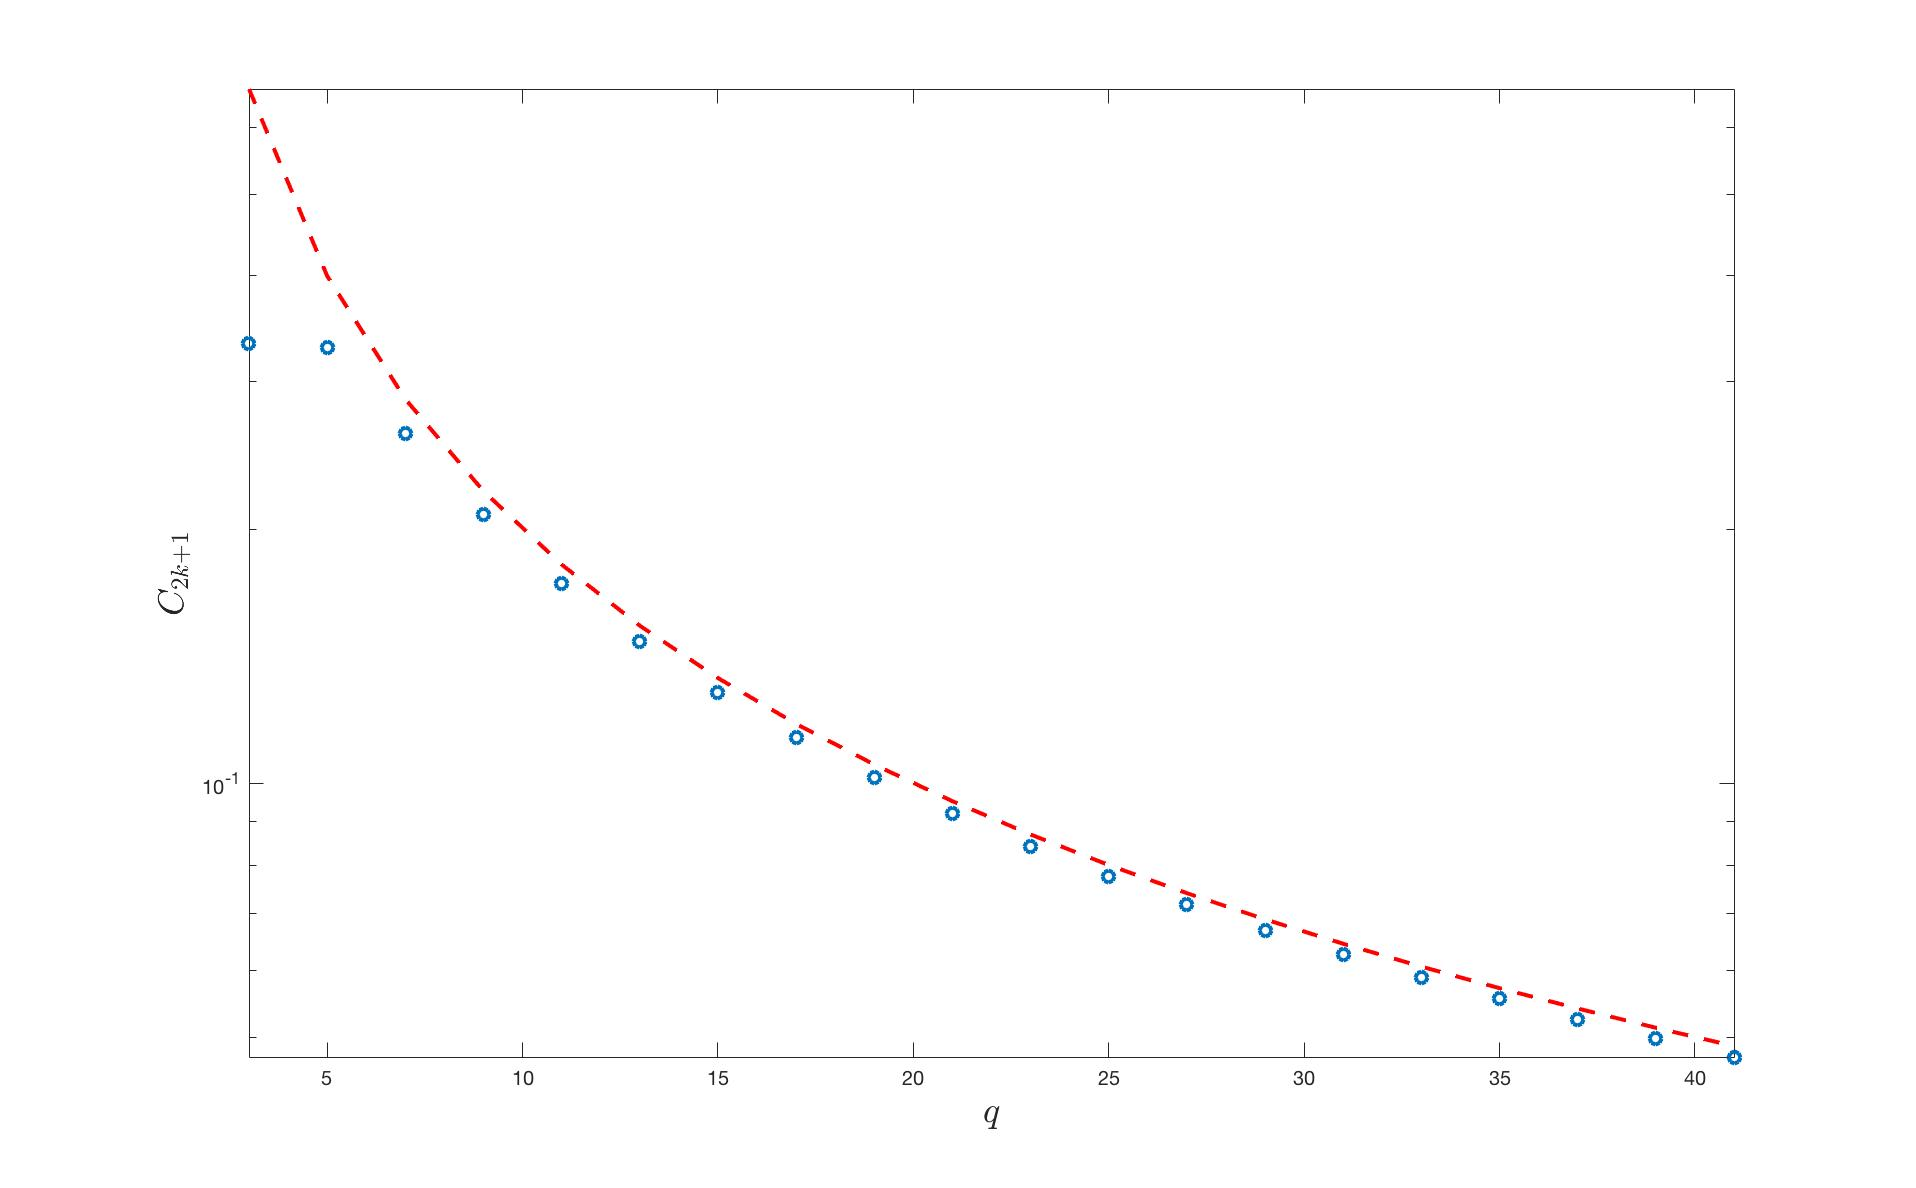
\includegraphics[width=0.8\linewidth]{Cqcome2suqcopy}
	\caption{The red dashes represent the function $\frac{2}{q}$; whereas the blu circles, the coefficients $C_q$ for odd $q$. The plot is realized setting $L=100$.}
	\label{fig:cqcome2suqcopy}
\end{figure}
\begin{figure}[h!]
	\centering
	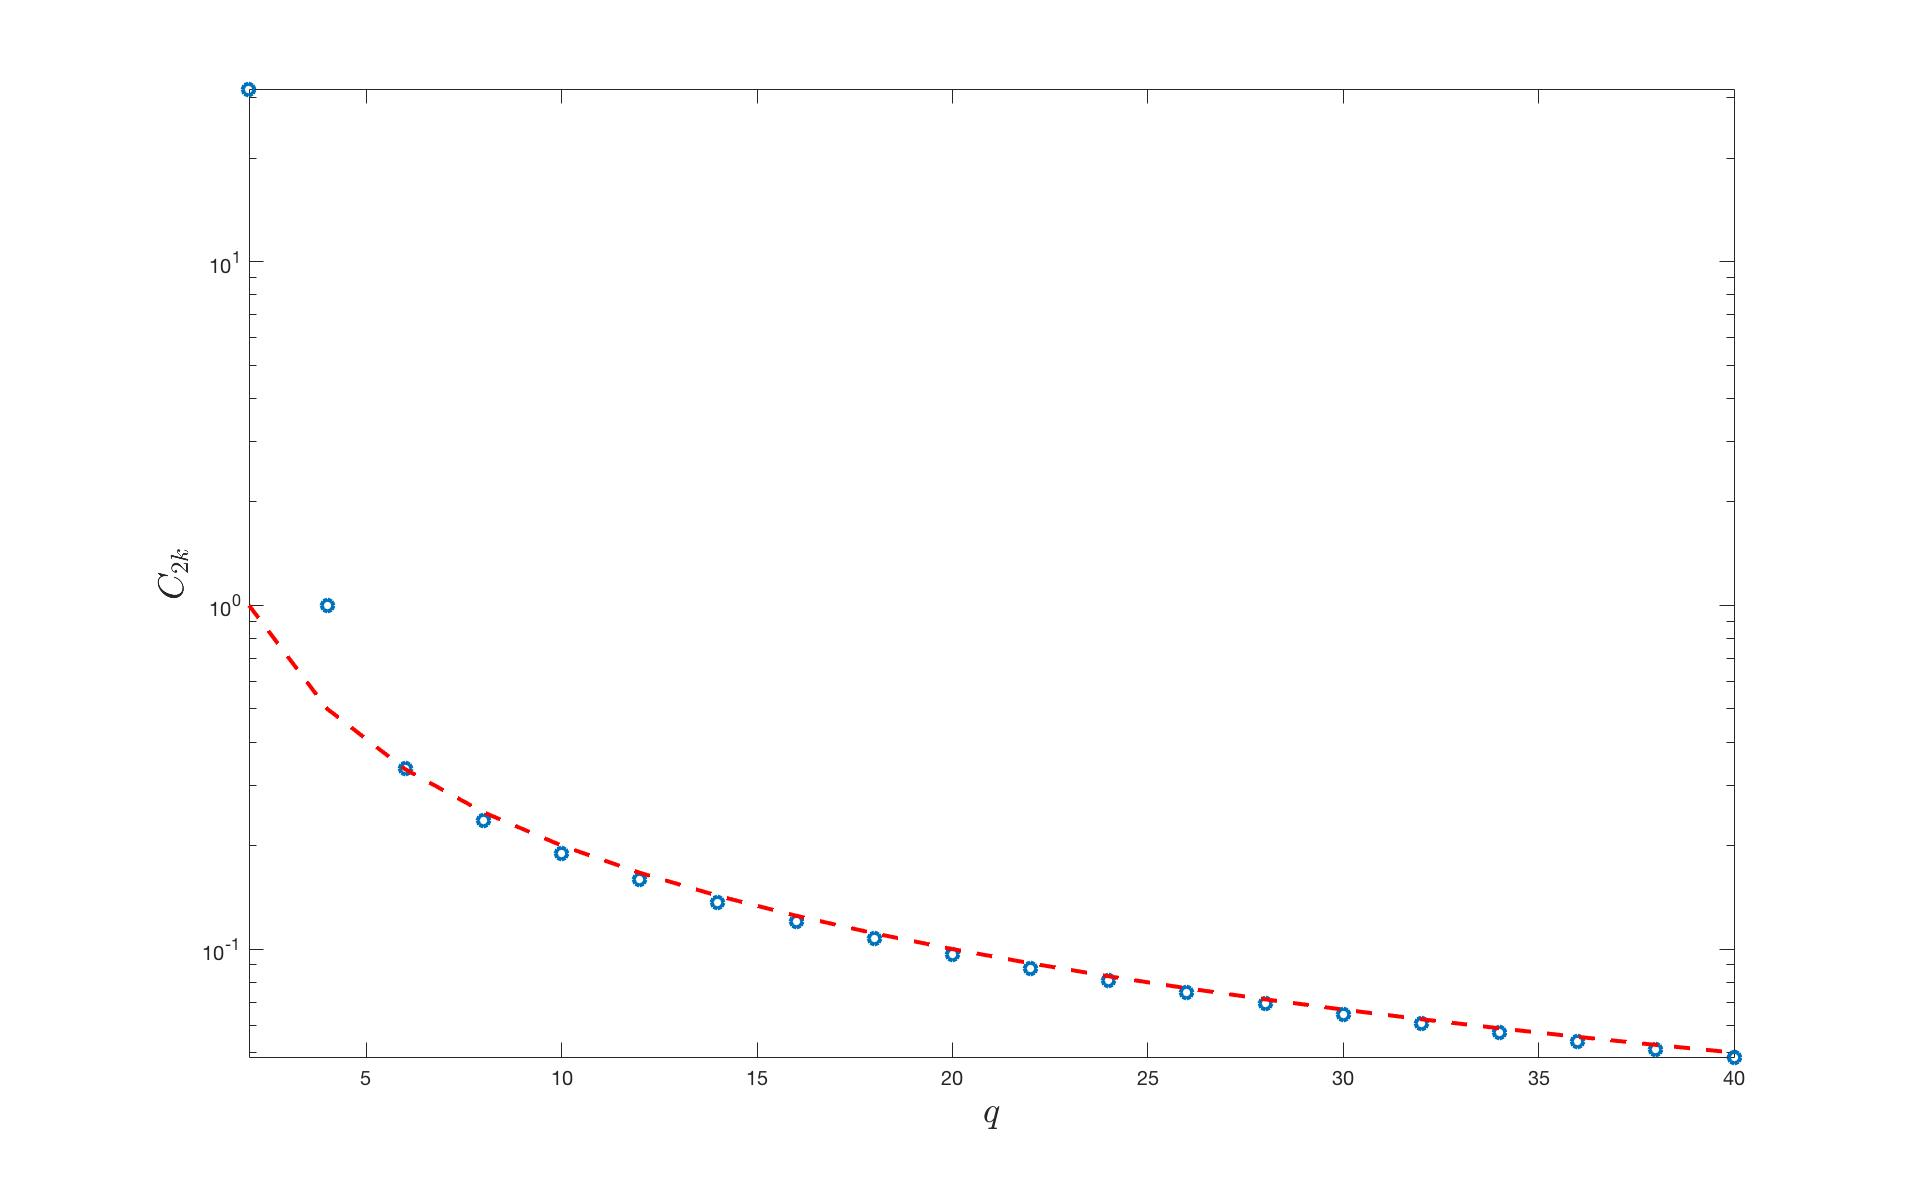
\includegraphics[width=0.8\linewidth]{C2k}
	\caption{The red dashes represent the function $\frac{2}{q}$; whereas the blu circles, the coefficients $C_q$ for even $q$. The plot is realized setting $L=100$.}
	\label{fig:c2k}
\end{figure}


\begin{figure}[h!]
	\centering
	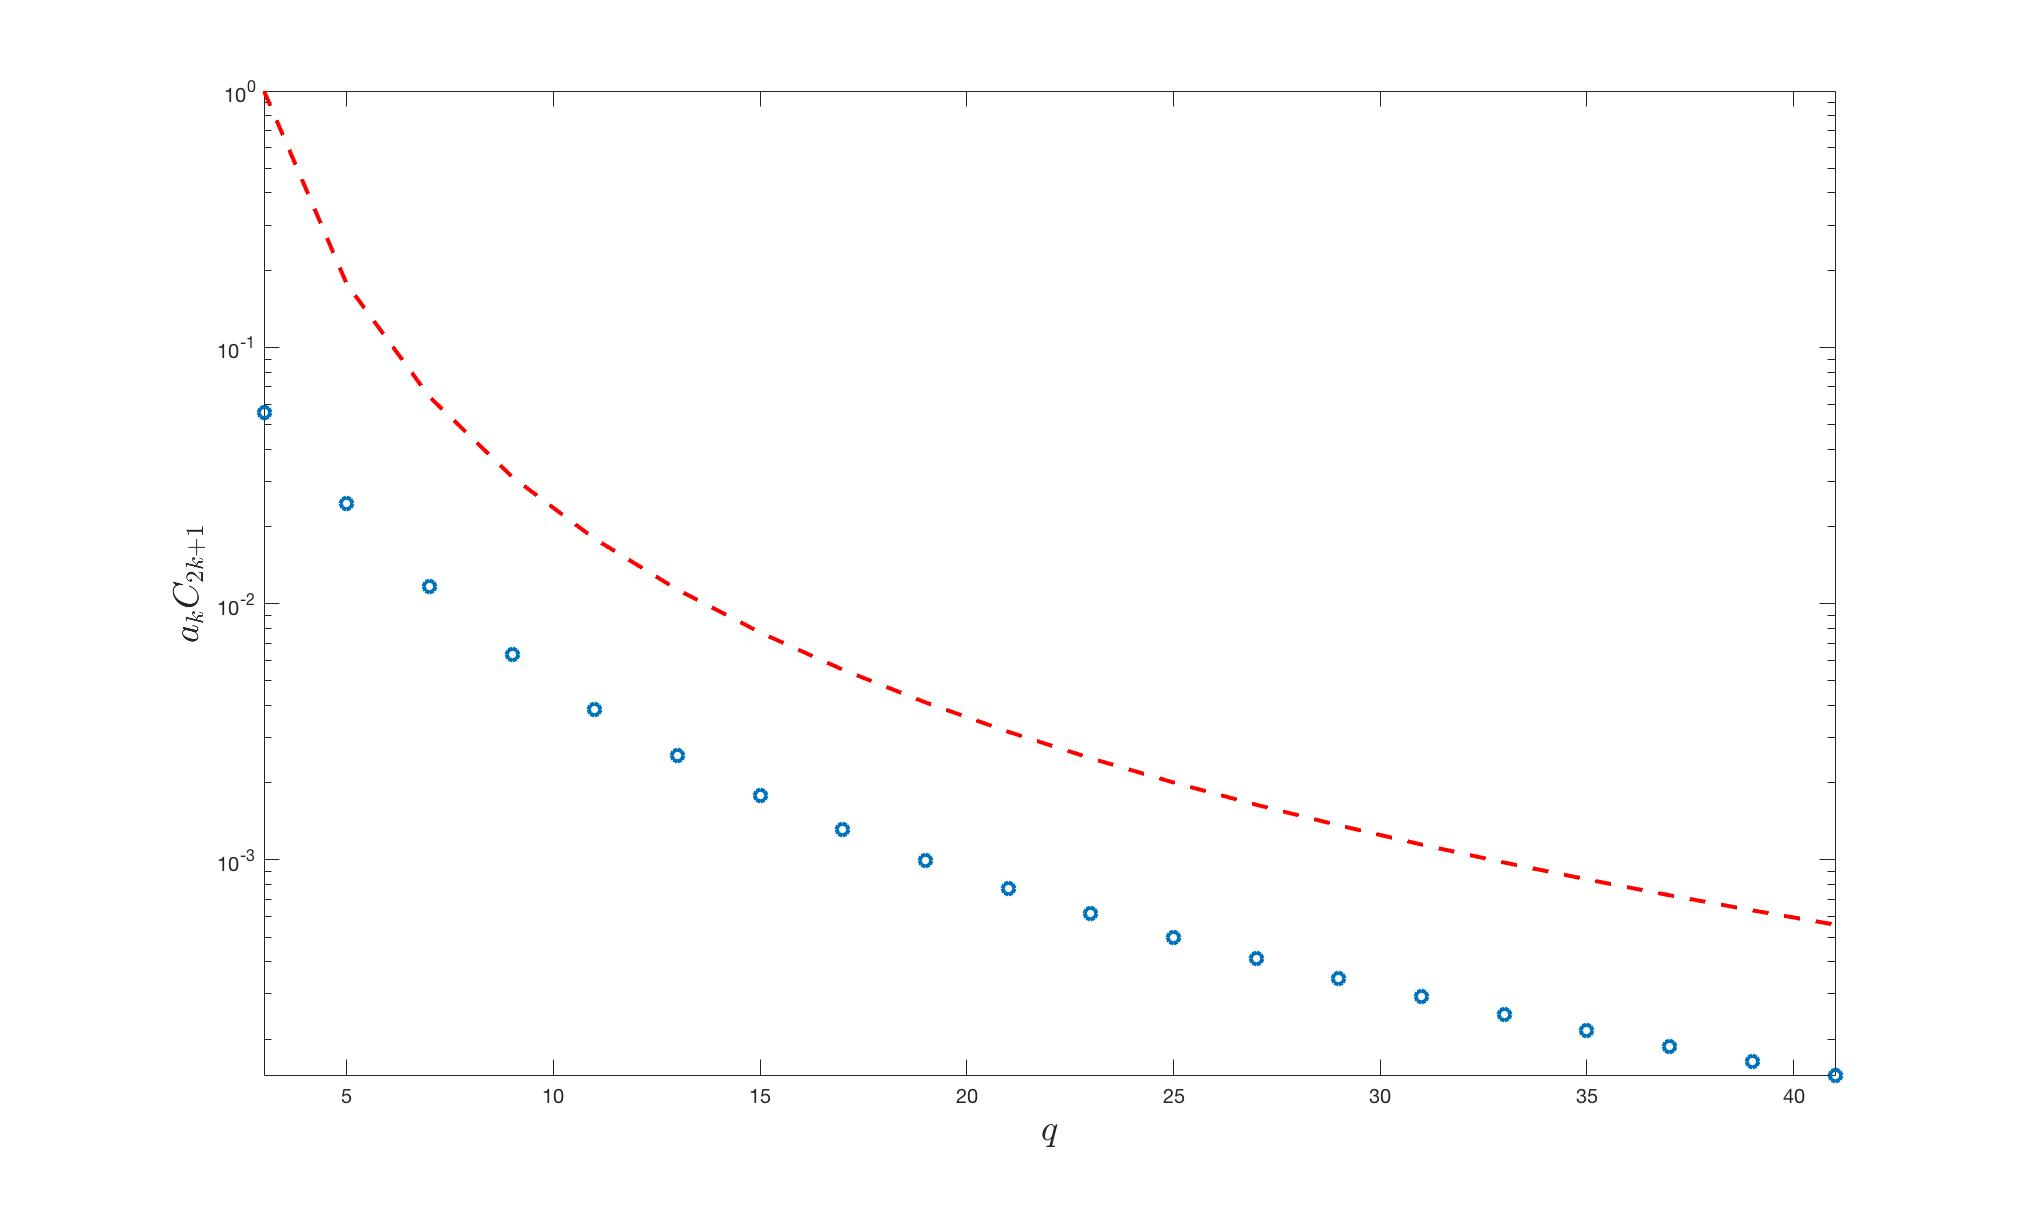
\includegraphics[width=0.8\linewidth]{akc2k1comeq5mezzi}
	\caption{The red dashes represents the function $\dfrac{1}{q^{5/2}}$; whereas the blue circles the points $a_kC_{2k+1}$. The plot is realized setting $L=100$.}
	\label{fig:akc2k1comeq5mezzi}
\end{figure}

\begin{remark}
	In \cite{MW2012}, the asymptotic behavior of the coefficients $a_k$ is proved to be $\dfrac{a}{k^{3/2}}$, where $a$ is a constant; then, in view of (\ref{Cq-approx}) the product $a_k C_{2k+1}$ has the same asymptotic behavior as $\dfrac{2a}{q^{5/2}}$. Indeed, Figure \ref{fig:akc2k1comeq5mezzi} compares the points $a_kC_{2k+1}$ with the function $\dfrac{1}{q^{5/2}}$.
\end{remark}


\begin{center}
\begin{tabular}{|c|c|c|c}
	\hline
	\textbf{LKC } &\textbf{	Mean } & \textbf{ Variance }\\
	\hline $\mathcal{L}_{2}(A_{u}(f_{\ell };\mathbb{S}^{2}))$ & $(1-\Phi(u)) $& $\dfrac{1}{8\pi} u^2 e^{-u^2} \dfrac{1}{\ell} + O(\dfrac{\log \ell}{\ell^2})$ \\
	\hline $\mathcal{L}_{1}(A_{u}(f_{\ell };\mathbb{S}^{2}))$ & $\dfrac{1}{2\sqrt{2}} e^{-u^2/2} \sqrt{\ell(\ell+1)}$ & $\dfrac{1}{128} u^4 e^{-u^2} \ell+O(\log \ell)$ \\
	\hline $\mathcal{L}_{0}(A_{u}(f_{\ell };\mathbb{S}^{2}))$  & $ \dfrac{1}{4\pi}\sqrt{\dfrac{2}{\pi}} e^{-u^2/2}u \dfrac{\ell(\ell+1)}{2}+\dfrac{1}{2\pi}(1-\Phi(u))$ & $\dfrac{1}{128\pi^3}u^2(u^2-1)^2 e^{-u^2} \ell^3+O(\ell^2 \log \ell)$ \\
	\hline
\end{tabular}
\end{center}

\begin{center}
\begin{tabular}{|c|c|c|c}
	\hline
	\textbf{ LKC  } &\textbf{	Mean } & \textbf{ Variance }\\
	\hline $\mathcal{L}_{2}(A_{u=0}(f_{\ell };\mathbb{S}^{2}))$ & $\dfrac{1}{2\pi} $& $  \frac{0.0188}{\ell^2}+o(\frac{1}{\ell^2})$  \\
	\hline $\mathcal{L}_{1}(A_{u=0}(f_{\ell };\mathbb{S}^{2}))$ & $\dfrac{1}{4\sqrt{2}} \sqrt{\ell(\ell+1)}$ & $\dfrac{1}{128} \dfrac{1}{16 \pi^2} \big\{ \log \ell+1.9542 \big\}+O(1)$ \\
	\hline $\mathcal{L}_{0}(A_{u=0}(f_{\ell };\mathbb{S}^{2}))$  & $\dfrac{1}{4\pi}$ & $O(\ell^2 \log \ell)$  \\
	\hline
\end{tabular}
\end{center}

We stress again that here $|\mathbb{S}^2|=1$, hence, to obtain these statistics when $|\mathbb{S}^2|=4\pi$ we need to multiply the mean for $4\pi$ and the variance for $16 \pi^2$, for the area and the Euler Poincar\'e characteristic. Whereas, for the boundary length ($=2\mathcal{L}_{1}(A_{u}(f_{\ell };\mathbb{S}^{2}))$) we need to multiply for $4\pi \times 2$ to compute the mean and for $ 16\pi^2 \times 4$ for the variance. The asymptotic behavior at $u=0$ of the Euler Poincar\'e characteristic is supposed to be $O(\ell^2 \log \ell)$ but the proof is still missing.\\\\
\begin{center}
\begin{tabular}{|c|c|c|c}
	\hline
	\textbf{ } &\textbf{	Mean } & \textbf{ Variance }\\
	\hline $\mathcal{N}^c(T_\ell)$ &$\frac{2}{\sqrt{3}} \ell^2+O(1)$ & $\frac{1}{3^3\pi^2} \ell^2 \log \ell +O(\ell^2)$ 
\\	\hline 
$\mathcal{N}_\ell^c(u,+\infty)$& $\frac{2}{\sqrt{8\pi}} \ell(\ell+1) \big\{ \frac{2}{\sqrt{6}}\Gamma(\frac{1}{2},\frac{3u^2}{2})+e^{-u^2/2}u\big\}$ &
$\frac{1}{2^5 \pi^3} \big\{ \frac{-2\sqrt{6}}{9} \Gamma(\frac{1}{2}, \frac{3u^2}{2})+\frac{2}{3} e^{-3/2u^2}u (1+19u^2)$ \\  & & 
 $-e^{-u^2/2}u(1+6u^2-u^4) \big\}^2 \ell^2 \log \ell +O(\ell^2)$\\
\hline
	\hline $\mathcal{N}_\ell^c(0,+\infty)$ & $\frac{1}{\sqrt{3}} \ell(\ell+1) +O(1)$ &  $\frac{1}{4 \pi^2 27} \ell^2 \log \ell+O(\ell^2)$\\
	\hline
\end{tabular}
\end{center}

where $$\Gamma(a,x)=\int_{x}^{\infty} t^{a-1}e^{-t}\,dt.$$

@@@

\section{Acknowledgments}
The authors acknowledge support from ERC Grant 277742 Pascal.
We acknowledge the use of resources from the
Norwegian national super-computing facilities, NOTUR. Maps and results
have been derived using the \healpix (http://healpix.jpl.nasa.gov)
software package developed by \cite{healpix}.

	\begin{thebibliography}{99}
	
	\bibitem{abra} Abramowitz, M.; Stegun, I. A. (1964) \textit{Handbook of mathematical functions with formulas, graphs, and mathematical tables}. National Bureau of Standards Applied Mathematics Series, 55 For sale by the Superintendent of Documents, U.S. Government Printing Office, Washington, D.C. 1964 xiv+1046 pp. (Reviewer: D. H. Lehmer) 33.00 (65.05)
	
	\bibitem{Adler-The} Adler R. J. (1981), \textit{The geometry of Random Fields}, Wiley and Sons, New York. 
	
	\bibitem{Adler e Taylor} Adler, R. J.; Taylor, J. E. (2007)
	\textit{Random fields and geometry}. Springer Monographs in Mathematics. Springer,
	New York.
	
	% \bibitem{ATW} Adler R. J., Taylor J. E. and Worsley K. J. (2010), \textit{Applications of random fields and geometry: Foundations and case studies}, Available at http://webee.technion.
	%	ac.il/people/adler/publications.html.
	\bibitem{AAR} Andrews G. E, Askey R., Roy R. (1999) \textit{Special Functions Enciclopedia of Mathematics and its Applications}, 71, Cambridge University Press, Cambridge.
	
	\bibitem{AH} Atkinson K., Han W. (2012) \textit{Spherical Harmonics and Approximations on the Unit Sphere: an introduction, Lecture Notes in Mathematics}, 2044, Springer.
	
	
	
	
	\bibitem{Azais e ws} Azais, J. M.; Wschebor, M. (2009) \textit{Level sets
		and extrema of random processes and fields}, Wiley and Sons, New Jersey.
	
	%	\bibitem{BBW} Benatar, J., Buckley, J., Wigman, I. Two applications of Bourgain's de-randomization method on toral eigenfunctions and spectral quasi-correlations, in preparation.
	
%	\bibitem{Baldi} Baldi, P. (2010) Representation of Gaussian isotropic spin random fields. \textit{Physical Review D, 81:083505}. Stochastic Process. Appl. 124 (2014), no. 5, 1910-1941.
	
	\bibitem{BKMP2009} Baldi, P.; Kerkyacharian, G.; Marinucci, D.; Picard, D. (2009). Asymptotics for Spherical Needlets, \textit{Annals of Statistics}, Vol. 37, No. 3, 1150-1171.
	
	\bibitem{BKMP} Baldi, P.; Kerkyacharian, G.; Marinucci, D.; Picard, D. (2009). Subsampling Needlet Coefficients on the Sphere, \textit{Bernoulli}, Vol. 15, 438-463.
	
	\bibitem{Baldi2} Baldi, P.; Trapani, S. (2015) Fourier coefficients of invariant random fields on homogeneous spaces of compact Lie groups, \textit{Ann. Inst. Henri Poincar\'e Probab. Stat. }51, no. 2, 648-671.
	
	
%	\bibitem{Barnett} Barnett, J. T. (2001). \textit{Zero-Crossings of Random Processes with Application to Estimation Detection}. In Marvasti, Farokh A. Nonuniform Sampling: Theory and Practice. Springer. ISBN 0306464454.
	
	\bibitem{BG} Beffara, V.; Gayet, D. (2017). Percolation of random nodal lines. Publ. \textit{Math. Inst. Hautes Etudes} Sci. 126, 131-176.
	
	\bibitem{BMW} Benatar, J.; Marinucci, D.; Wigman I. (2017) Planck-scale distribution of nodal length of arithmetic random waves, preprint,
	arXiv:1710.06153.
	
	\bibitem{berard} Berard, P. (1985) Volume des ensembles nodaux des fonctions propres du laplacien. (French) [Volume of the nodal sets of eigenfunctions of the Laplacian] Bony-Sjöstrand-Meyer seminar, 1984–1985, Exp. No. 14 , 10 pp., École Polytech., Palaiseau, 1985. 
	
	\bibitem{berry} Berry, M. V. (2002) Statistics of nodal lines and points in chaotic quantum billiards: perimeter corrections, fluctuations, curvature, \textit{J. Phys. }A 35, no. 13, 3025–3038. 
	
	\bibitem{Berry1977} Berry, M. V. (1977) Regular and irregular semiclassical wavefunctions. \textit{J. Phys.} A 10, no. 12, 2083–2091. 81.58.
	
	\bibitem{BSZ} Bleher, P.; Shiffman, B.; Zelditch, S. (2000) Universality and scaling of correlations between zeros on complex manifolds \textit{Invent. Math.} 142, no. 2, 351-395.
	
	\bibitem{BSZ2} Bleher, P.; Shiffman, B.; Zelditch, S. (2001). Universality and scaling of zeros on symplectic manifolds Random matrix models and their applications, 31-69, \textit{Math.Sci. Res. Inst. Publ.}, 40, Cambridge Univ. Press, Cambridge.
	
	%	\bibitem{Bo}  Bourgain, J. On toral eigenfunctions and the random wave model. Israel \textit{J. of Math.} 201, no. 2 (2014): 611-630.
	
	%	\bibitem{Br}  Br\"{u}ning, J. Uber Knoten Eigenfunktionen des Laplace-Beltrami Operators, Math. Z.	158 (1978), 15-21.
	
	%\bibitem{BG} Br\"{u}ning, J.; Gromes, D. Uber die L\"{a}nge der Knotenlinien schwingender Membranen, Math. Z. 124 (1972), 79-82.
	
	\bibitem{BR11} Bourgain, J., Rudnick, Z. (2011) On the geometry of the nodal lines of eigenfunctions on the two-dimensional torus,\textit{ Ann.
		Henri Poincar\'e }12, no. 6, 1027-1053.
	
	\bibitem{brockwell and davis} Brockwell, P. J.; Davis, R. A. (1996) \textit{Introduction to Time Series and Forecasting}, Springer-Verlag, New York, Inc.
	
	
	\bibitem{BW2016} Buckley, J.; Wigman, I. (2016)
	On the number of nodal domains of toral eigenfunctions. (English summary),
	\textit{Ann. Henri Poincar\'e 17}, no. 11, 3027-3062.
	
	%\bibitem{C2014} Chatterjee, Sourav A short survey of Stein's method. Proceedings of the International Congress of Mathematicians Seoul 2014. Vol. IV, 1-24, Kyung Moon Sa, Seoul, 2014.
	
	%	\bibitem{C2008}	Sourav Chatterjeear, A new method of normal approximation. Xiv:math/0611213.
	
	\bibitem{C} Cammarota, V. (2017) Nodal Area Distribution For Arithmetic Random
	Waves, arXiv:1708.07679v1.
	
	
	\bibitem{CM}  Cammarota, V.; Marinucci, D. (2018) A Quantitative Central Limit Theorem for the Euler-Poincaré Characteristic of Random Spherical Eigenfunctions. \textit{Annals of Probabability }46, no. 6, 3188–3228.
	
	\bibitem{CM2015} Cammarota, V.; Marinucci, D., (2015) On the limiting behavior of Needlets Plyspectra, (English, French summary) 
	\textit{Ann. Inst. Henri Poincaré Probab. Stat.} 51, no. 3, 1159–1189. 
	
	\bibitem{CMW} Cammarota, V.; Marinucci, D.; Wigman, I. (2016) Fluctuations of the Euler-Poincar\'e characteristic for random spherical harmonics,
	\textit{Proceedings of the American Mathematical Society}, 11, 4759-4775.
	
	
	
	\bibitem{CMW2016} Cammarota, V.; Marinucci, D.; Wigman, I. (2016) On the distribution of the critical values of random spherical harmonics,
	\textit{Journal of Geometric Analysis}, 4, 3252-3324.
	
	
	\bibitem{C2009} Chatterjee, S. (2009) Fluctuations of eigenvalues and second order Poincar\'e inequalities. \textit{Probab. Theory Related Fields} 143, no. 1-2, 1–40. 
	
%	\bibitem{cheng} Cheng, D. (2017) Excursion probabilities of isotropic and locally isotropic gaussian random fields on manifolds, \textit{Extremes} 20, no. 2, 475–487.
	
	
%	\bibitem{cheng2} Cheng, D. (2015) Excursion probability of certain non-centered smooth gaussian random fields, Preprint (ArXiv 1502.04414).
	
	\bibitem{Cheng} Cheng, S. Y. (1976) Eigenfunctions and nodal sets, 	\textit{Comm. Math. Helv.} 51, no. 1, 43–55. 
	
	
%	\bibitem{CS}Cheng, D.; Schwartzman, A. (2015) On the explicit height distribution and expected number of local maxima of isotropic gaussian random fields, Preprint (ArXiv1503.01328).
	
%	\bibitem{CX} Cheng, D.; Xiao, Y. (2012) The mean euler characteristic and excursion probability of gaussian random fields with stationary increments, Preprint (ArXiv 1211.6693).
	
	%	\bibitem{Mau 2014} Cheng, D.; Xiao, Y. (2016) Excursion probability of gaussian random fields on sphere, \textit{Bernoulli} 22, no. 2, 1113–1130.
	
	
	\bibitem{cramer and leadbetter} Cramér, H.; Leadbetter, M. R. (1967), \textit{Stationary and related stochastic processes}, Wiley, New York.
	
	
	\bibitem{DNPR} Dalmao, F.; Nourdin, I.; Peccati, G.; Rossi, M. (2016) Phase Singularities in Complex	Arithmetic Random Waves. arXiv:1608.05631v3.
	
	\bibitem{DF} Donnelly, H.; Fefferman, C.  (1988) Nodal sets of eigenfunctions on Riemannian manifolds,
	\textit{ Invent. Math.} 93, 161-183.
	
	\bibitem{FHMM} Fantaye, Y.; Hansen, F.K.; Maino, D.; Marinucci, D. (2015) Cosmological Applications of the Gaussian Kinematic Formula, \textit{Physical Review D}, Volume 91, 063501.
	
	\bibitem{GM} Geller, D.; Mayeli, A. (2009) Continuous Wavelets on Manifolds, \textit{Math. Z.}, Vol. 262, pp. 895-927.
	
	\bibitem{GW16}  Granville, A.; Wigman, I. (2017) Planck-scale mass equidistribution of toral Laplace eigenfunctions. \textit{Comm. Math. Phys.}, 355, no. 2, 767–802.
	
	\bibitem{KKW} Krishnapur, M.; Kurlberg P.; Wigman, I. (2013) Nodal length
	fluctuations for arithmetic random waves. \textit{Annals of Mathematics} (2)
	177, no. 2, 699-737.
	
	
	
%	\bibitem{KW} Krishnapur M.; Wigman I. Fluctuations of the nodal length of random eigenfunction of the Laplace ont he torus.  
	
	\bibitem{LMX} 
	Lan, X.; Marinucci, D.; Xiao, Y. (2018) Strong local nondeterminism and exact modulus of continuity for spherical Gaussian fields.
	\textit{Stochastic Process. Appl.} 128, no. 4, 1294-1315. 
	
	
	\bibitem{Lang e Schwab} Lang, A.; Schwab, C. (2015) Isotropic Gaussian random fields on the sphere: regularity, fast simulation and stochastic partial differential equations. \textit{Ann. Appl. Probab.} 25, no. 6, 3047-3094.
	
	\bibitem{LeRu}  Lester, S.; Rudnick, Z. (2017) Small scale equidistribution of eigenfunctions on the torus, \textit{Comm. Math. Phys.}, 350 (1), 279-300.
	
	\bibitem{13} Lewis, A. (2012) The full squeezed CMB bispectrum from inflation. \textit{Journal of Cosmology and Astroparticle Physics}, 06, 023. 
	
	\bibitem{Logunov b} Logunov, A. (2018) Nodal sets of Laplace eigenfunctions: polynomial upper estimates of the Hausdorff measure. \textit{Ann. of Math.} (2) 187, no. 1, 221-239.
	
	\bibitem{Logunov a} Logunov, A. (2018) Nodal sets of Laplace eigenfunctions: proof of Nadirashvili's conjecture and of the lower bound in Yau's conjecture. \textit{ Ann. of Math. }(2) 187, no. 1, 241-262.
	
	\bibitem{LM} Logunov, A.; Malinnikova, E. (2015) On ratios of harmonics functions. \textit{Adv. Math.} 274, 241-262. 
	
	
	%	\bibitem{Malyarenko1}Malyarenko, A. Invariant random fields in vector bundles and application to cosmology, Ann. Inst. Henri Poincar´e Probab. Stat. 47 (2011), no. 4, 1068?1095. MR 2884225 (2012k:60151)
	
	
	%	\bibitem{Malyarenko2}, Invariant random fields on spaces with a group action, Probability and its Applications (New York), Springer, Heidelberg, 2013, With a foreword by Nikolai Leonenko. MR 2977490
	\bibitem{M2008} Marinucci, D. (2008) A Central Limit Theorem and Higher Order Results for the Angular Bispectrum, \textit{Probability Theory and Related Fields}, Vol. 141, N.3-4, pp. 389-409, math.pr/0509430.
	
	\bibitem{M2006} Marinucci, D. (2006) High Resolution Asymptotics for the Angular Bispectrum of Spherical Random Fields, \textit{Annals of Statistics}, Vol.34, N.1, pp. 1-4.
	
	\bibitem{Marinucci} Marinucci, D. (2015) Lecture Notes on Spherical Random Fields. Lecture notes, Finnish School in Probability and Statistics, June 2015.
	
	
	\bibitem{M e P 2013} Marinucci, D.; Peccati, G. (2013) Mean-square continuity on homogeneous spaces of compact groups. (English summary) 
	\textit{Electron. Commun. Probab.} 18, no. 37, 10 pp.
	
	\bibitem{M e Peccati}  Marinucci, D.; Peccati, G. (2011) \textit{Random fields on the sphere. Representation, limit theorems and cosmological applications}. London Mathematical Society Lecture Note Series, 389. Cambridge University Press, Cambridge. 
	
	
	\bibitem{MPRW} Marinucci, D.; Peccati, G.; Rossi, M.; Wigman, I. (2016)
	Non-universality of nodal length distribution for arithmetic random waves. (English summary)
	\textit{Geom. Funct. Anal.} 26, no. 3, 926-960.
	
	\bibitem{M e Mau 2015} Marinucci, D.; Rossi, M. (2015) Stein-Malliavin approximations for nonlinear functionals of random eigenfunctions on $\mathbb{S}^d$. \textit{J. Funct. Anal. }268, no. 8, 2379-2420. 
	
	%	\bibitem{MRW} Marinucci D., Rossi M., Wigman I. Nodal length of random spherical harmonics (2017) arXiv:1705.05747.
	
	
	\bibitem{MRW2017} Marinucci, D.; Rossi, M.; Wigman, I. (2017) The asymptotic
	equivalence of the sample trispectrum and the nodal length for random
	spherical harmonics, preprint, arXiv:1705.05747.
	
	
%	\bibitem{M e Vadlamani} Marinucci, D.; Vadlamani, S. (2015) A note on global suprema of band-limited spherical random functions. \textit{Statist. Probab. Lett.} 96, 141-148.
	
	
	\bibitem{MV} Marinucci, D.; Vadlamani, S. (2016) High-Frequency Asymptotics for Lipschitz-Killing Curvatures of Excursion Sets on the Sphere. \textit{Ann. Appl. Probab.} 26, no. 1, 462-506. 
	
	
	
	\bibitem{M e W 2012} Marinucci, D.; Wigman, I. (2014) On nonlinear functionals of
	random spherical eigenfunctions. \textit{Comm. Math. Phys.} 327, no. 3,
	849-872.
	
	\bibitem{M e W 2011} Marinucci, D.; Wigman, I. (2011) On the excursion sets of spherical Gaussian eigenfunctions. \textit{J. Math. Phys.} 52, no. 9, 093301, 21 pp.
	
	\bibitem{M e W 2011bis} Marinucci, D.; Wigman, I. (2011) The Defect Variance of Random Spherical Harmonics. \textit{Journal of Physics A: Mathematical and Theoretical}, 44, 355206.
	
	\bibitem{Matsubara} Matsubara, T. (2010) Analytic Minkowski functionals of the Cosmic Microwave Background: second-order non-Gaussianity with bispectrum and trispectrum. \textit{Phys. Rev. D} 81, 083505.
	
	\bibitem{NPW2} Narcowich, F. J.; Petrushev, P.; Ward, J.D. (2006) Decomposition of Besov and Triebel-Lizorkin spaces on the sphere, \textit{Journal of Functional Analysis}, 238, 2, 530-564.
	
	\bibitem{NPW} Narcowich, F. J.; Petrushev, P.; Ward, J.D. (2006) Localized tight frames on spheres, \textit{SIAM Journal of Mathematical Analysis}, 38, 2, 574-594.
	
	
	
	\bibitem{N} Neuheisel, J. (2000) The asymptotic distribution of nodal sets on spheres, Johns Hopkins
	Ph.D. thesis.
	
	\bibitem{Peccati Nourdin} Nourdin, I.; Peccati, G. (2012) \textit{Normal approximations with Malliavin calculus. From Stein's method to universality.} Cambridge Tracts in Mathematics, 192. Cambridge University Press, Cambridge. 
	
	\bibitem{NP2009} Nourdin, I.; Peccati, G. (2010) Stein's method meets Malliavin calculus: a short survey with new estimates. Recent development in stochastic dynamics and stochastic analysis, 207–236, \textit{Interdiscip. Math. Sci.}, 8, World Sci. Publ., Hackensack, NJ, 2010.
	
	\bibitem{NPR} Nourdin, I.; Peccati, G.; Rossi, M. (2017) Nodal Statistics of
	Planar Random Waves. arXiv:1708.02281v1.
	
	
	
	%\bibitem{ORW} Oravecz, F., Rudnick, Z., Wigman, I. The Leray measure of nodal sets for random eigenfunctions on the torus, Ann. Inst. Fourier (Grenoble) 58 (2008), 299-335.
	
	
	
	
	
	%\bibitem{M e W 2011bis} Domenico Marinucci and Igor Wigman (2011), The Defect Variance of Random Spherical Harmonics,
	%Journal of Physics A: Mathematical and Theoretical, 44, 355206.
	
	
	\bibitem{PR2017} Peccati, G.; Rossi, M. (2017). Quantitative limit theorems for local functionals of arithmetic random waves. \textit{Computation and Combinatorics in Dynamics, Stochastics and Control, The Abel Symposium 2016} – Springer (in press).  arXiv:1702.03765v1.
	
	\bibitem{PTudor}Peccati, G.; Tudor, C.A. (2007) Anticipating integrals and martingales on the Poisson space, \textit{Random Oper. Stoch. Equ.} 15, no. 4, 327–352. 
	
%	\bibitem{P e T} Peccati, G.; Taqqu, M.S. (2011) Wiener Chaos: Moments, Cumulants and Diagrams, Springer-Verlag.
	
	\bibitem{Planck 2015} Planck 2013 results. XXIV. Constraints on primordial non-Gaussianity (Planck Collaboration), \textit{Astronomy and Astrophysics},  Volume 571, idA24, 58 pp. (2014).
	
	\bibitem{Planck 2014} Planck 2013 results. XXIII. Isotropy and statistics of the CMB (Planck Collaboration), \textit{Astronomy and Astrophysics},  Volume 571, idA23. (2014)
	
	\bibitem{Rossi2} Rossi, M. (2018) Random Nodal Lengths and
	Wiener Chaos. \textit{Proceedings of the Workshop “Probabilistic Methods in Spectral Geometry and PDE” in Montréal, August 2016} (to appear). arXiv:1803.09716.
	
	\bibitem{Rossi} Rossi, M. (2016) The defect of random hyperspherical harmonics, \textit{Journal of Theoretical Probability} (in press). arXiv:1605.03491.
	
	
	\bibitem{mau} Rossi, M. (2016) The geometry of spherical random fields - PhD thesis. arXiv:1603.07575.
	
	
	%\bibitem{Rossi} Rossi On the high-energy defect distribution for random hyperspherical harmonics
	

	
	\bibitem{RossiW} Rossi, M.; Wigman, I. (2018) Asymptotic distribution of nodal intersections for arithmetic random waves. \textit{Nonlinearity} 31, no. 10, 4472-4516. 
	
	
	
	\bibitem{RW} Rudnick, Z.; Wigman I. (2016) Nodal intersections for random
	eigenfunctions on the torus, \textit{American Journal of Mathematics}, 138, no. 6,
	1605-1644.
	
	\bibitem{RW2} Rudnick, Z.; Wigman, I. (2008) On the volume of nodal sets for eigenfunctions of the Laplace on the torus, \textit{annales Henri Poincar\'e}, Vol.9, No 1, 109-130.
	
	\bibitem{RWY} Rudnick, Z.; Wigman, I.; Yesha N. (2015) Nodal intersections for
	random waves on the 3-dimensional torus, \textit{Annales Institut Fourier}, 66, no.
	6, 2455-2484.
	
	\bibitem{Schoenberg (1942)}Schoenberg, I.J. (1942) Positive definite functions on spheres. \textit{Duke math. J.} 9, 96-108.
	
	
	
	\bibitem{szego} Szego, G. (1975) Orthogonal polynomials, Fourth edition. \textit{%
		American Mathematical Society, Colloquium Publications, Vol. XXIII.} \textit{%
		American Mathematical Society, Providence, R.I.}
	
	\bibitem{AP1} Todino, A. P. (2018) A Quantitative Central Limit Theorem for the Excursion Area of
	Random Spherical Harmonics over Subdomains of $\mathbb{S}^2$. arXiv:1807.06982
	
	\bibitem{AP2} Todino, A. P. (2018) Nodal Lengths in Shrinking Domains for Random Eigenfunctions on $\mathbb{S}^2$. arXiv:1807.11787.
	
%	\bibitem{Triebel} Triebel, H. (1995). \textit{Interpolation Theory, Function Spaces, Differential Operators}, 2nd ed. Johann Ambrosius Barth, Heildelberg.
	
%	\bibitem{TW} Toth John A.; Wigman I. (2009) Universality of length distribution of nodal lines of random waves on generic surfaces.
	
	%\bibitem{VMK} Varshalovich D.A., A.N. Moskalev, and Khersonskii V.K. (1988), Quantum Theory of Angular Momentum, World Scientific.
	
	\bibitem{quantum theory} Varshalovich, D. A.; Moskalev, A. N.; Khersonski,
	V. K. (1988) \textit{Quantum theory of angular momentum. Irreducible tensors,
		spherical harmonics, vector coupling coefficients, 3nj symbols}. Translated
	from the Russian. World Scientific Publishing Co., Inc., Teaneck, NJ.
	
	
	
	
	\bibitem{Wigman2} Wigman, I. (2011) On the nodal lines of random and deterministic Laplace eigenfunctions, \textit{Spectral geometry}, \textit{Proc. Sympos. Pure Math.}, vol. 84, \textit{Amer. Math. Soc.}, \textit{Providence, RI}, 2012, pp. 285-297. 
	
	\bibitem{W} Wigman, I. 	(2010) Fluctuations of the nodal length of random spherical
	harmonics, \textit{Communications in Mathematical Physics, 398 no. 3 787-831}.
	
	\bibitem{35} Wigman, I. (2009) On the distribution of the nodal sets of random
	spherical harmonics. \textit{Journal of Mathematical Physics}, 50, no. 1,
	013521, 44 pp.
	
%	\bibitem{W1} Wigman I., Volume fluctuations of the nodal sets of random Gaussian subordinated spherical harmonics.
	
	
	
	
	
	% \bibitem{RW} Rudnick, Z., Wigman I.; Nodal intersections for random eigenfunctions on the torus, \textit{American Journal of Mathematics, 138, no. 6}, 1605-1644 (2016).
	
	
	%\bibitem{mau} Maurizia Rossi(2015), the defect of random hyperspherical harmonics
	
	%\bibitem{szego} Szego Gabor (1975), Orthogonal polynomials, Fourth edition. American Mathematical Society, Colloquium Publications, Vol. XXIII. American Mathematical Society, Providence, R.I.
	
	%\bibitem{quantum theory} D.A Varshalovich, A.N. Moskalev, V.K. Khersonskii (1988), Quantum theory of angular momentum, World Scientific.
	
	
	\bibitem{Y1982}  Yau, S.T. (1982) Survey on partial differential equations in differential geometry. Seminar
	on Differential Geometry, pp. 3-71, \textit{Ann. of Math. Stud.}, 102, Princeton Univ. Press,
	Princeton, N.J.
	
	\bibitem{Y1990} Yau, S.T. (1993) Open problems in geometry. Differential geometry: partial differential equations
	on manifolds (Los Angeles, CA, 1990), 1-28, \textit{Proc. Sympos. Pure Math.}, 54,
	Part 1, \textit{Amer. Math. Soc.}, \textit{Providence, RI}.
	
%	\bibitem{Ylvisaker} Ylvisaker N. D. (1965). The Expected Number of Zeros of a Stationary Gaussian Process. \textit{The Annals of Mathematical Statistics.} 36 (3): 1043. doi:10.1214/aoms/1177700077.
	
	
	
	
	%	\bibitem{Wigman1}Igor Wigman, Fluctuations of the nodal length of random spherical harmonics, Comm. Math. Phys. 298 (2010), no. 3, 787?831. MR 2670928 (2012f:58073)
	
	
	%\bibitem{mall}Normal approximations with Malliavin calculus. 

\end{thebibliography} 

%\bibliography{mf_literature_wabstract,Planck_bib}

%\bibliography{gkf_proj2}



\end{document}

%%% Local Variables:
%%% mode: latex
%%% TeX-master: t
%%% End:
